% Manuscript prepared on top of the MDPI LaTeX template.
% Build (from manuscript/):
%   latexmk -pdf -bibtex -interaction=nonstopmode main.tex

%=================================================================
\documentclass[photonics,article,submit,pdftex,moreauthors]{Definitions/mdpi}
%\documentclass[preprints,article,submit,pdftex,moreauthors]{Definitions/mdpi}
% For posting an early version of this manuscript as a preprint, you may use "preprints" as the journal. Changing "submit" to "accept" before posting will remove line numbers.

%--------------------
% Class Options:
%--------------------
%----------
% journal
%----------
% Choose between the following MDPI journals:
% accountaudit, acoustics, actuators, addictions, adhesives, adolescents, aerobiology, aerospace, agriculture, agriengineering, agrochemicals, agronomy, ai, aichem, aieng, aimater, aimed, aipa, air, aisens, algorithms, allergies, alloys, amh, analog, analytica, analytics, anatomia, anesthres, animals, antibiotics, antibodies, antioxidants, applbiosci, appliedchem, appliedmath, appliedphys, applmech, applmicrobiol, applnano, applsci, aquacj, architecture, arm, arthropoda, asc, asi, astronautics, astronomy, atmosphere, atoms, audiolres, automation, axioms, bacteria, batteries, bdcc, beverages, biochem, bioengineering, biologics, biology, biomass, biomechanics, biomed, biomedicines, biomedinformatics, biomimetics, biomolecules, biophysica, bioresourbioprod, biosensors, biosphere, biotech, birds, blockchains, bloods, blsf, brainsci, breath, buildings, cancers, carbon, cardio, cardiogenetics, cardiovascmed, catalysts, cells, ceramics, challenges, chemengineering, chemistry, chemosensors, chemproc, children, chips, cimb, civileng, cleantechnol, climate, clinbioenerg, clinpract, clockssleep, cmd, cmtr, coasts, coatings, colloids, colorants, commodities, complexities, complications, compounds, computation, computers, condensedmatter, conservation, constrmater, cosmetics, covid, crops, cryo, cryptography, crystals, csmf, ctn, culture, curroncol, cyber, dairy, data, ddc, dentistry, dermato, dermatopathology, designs, devices, dhi, diabetology, diagnostics, dietetics, digital, disabilities, diseases, diversity, dna, drones, dynamics, earth, ebj, ecm, ecologies, edm, eesp, electricity, electrochem, electronicmat, electronics, encyclopedia, endocrines, energies, eng, engproc, entomology, entropy, environments, environremediat, epidemiologia, epigenomes, esa, est, fermentation, fibers, fintech, fire, fishes, fluids, foods, forecasting, forensicsci, forests, fossstud, foundations, fractalfract, fuels, future, futureinternet, futurepharmacol, futurephys, futuretransp, galaxies, gases, gastroent, gastrointestdisord, gastronomy, gels, genes, geographies, geohazards, geomatics, geometry, geosciences, geotechnics, geriatrics, germs, glacies, grasses, green, greenhealth, gucdd, hardware, hazardousmatters, healthcare, hearts, hemato, hematolrep, hep, heritage, higheredu, highthroughput, horticulturae, hospitals, hydrobiology, hydrogen, hydrology, hydropower, hygiene, idr, iic, ijem, ijerph, ijgi, ijmd, ijms, ijns, ijom, ijpb, ijt, ijtm, ijtpp, ime, immuno, informatics, information, infrastructures, inorganics, insects, instruments, inventions, iot, j, jaestheticmed, jal, jcdd, jcm, jcp, jcrm, jcs, jcto, jdad, jdb, jdream, jemr, jeta, jfb, jfmk, jgbg, jgg, jimaging, jlpea, jmahp, jmmp, jmms, jmp, jmse, jne, jnt, jof, joi, joitmc, joma, jop, joptm, jor, jox, jpbi, jphytomed, jpm, jsan, jtaer, jvd, jzbg, kidneydial, kinasesphosphatases, knowledge, labmed, laboratories, lae, land, life, lights, limnolrev, lipidology, liquids, livers, logics, logistics, lubricants, lymphatics, machines, macromol, magnetism, magnetochemistry, make, marinedrugs, materials, materproc, mathematics, mca, measurements, medicina, medicines, medsci, membranes, merits, metabolites, metals, meteorology, methane, metrics, metrology, micro, microarrays, microbiolres, microelectronics, micromachines, microorganisms, microplastics, microwave, minerals, mining, mmphys, modelling, molbank, molecules, mps, msf, mti, multimedia, muscles, nanoenergyadv, nanomanufacturing, nanomaterials, ncrna, ndt, network, neuroglia, neuroimaging, neurolint, neurosci, nitrogen, notspecified, nursrep, nutraceuticals, nutrients, obesities, occuphealth, oceans, ohbm, onco, optics, oral, organics, organoids, osteology, oxygen, pandemics, parasites, parasitologia, particles, pathogens, pathophysiology, pediatrrep, pets, pharmaceuticals, pharmaceutics, pharmacoepidemiology, pharmacy, philosophies, photochem, photonics, phycology, physchem, physics, physiologia, plants, plasma, platforms, pollutants, polymers, polysaccharides, populations, poultry, powders, precipitation, precisoncol, preprints, proceedings, processes, prosthesis, proteomes, psf, psychiatryint, psychoactives, purification, quantumrep, quaternary, qubs, radiation, rdt, reactions, realestate, receptors, recycling, regeneration, remotesensing, reports, reprodmed, resources, rheumato, rjpm, robotics, rsee, ruminants, safety, sci, scipharm, sclerosis, seeds, sensors, separations, sexes, shi, signals, sinusitis, siuj, skins, smartcities, sna, societies, software, soilsystems, solar, solids, spectroscj, sports, standards, stats, std, stratsediment, stresses, surfaces, surgeries, suschem, sustainability, symmetry, synbio, systems, tae, targets, taxonomy, technologies, telecom, test, textiles, thalassrep, therapeutics, thermo, timespace, tomography, toxics, toxins, tph, transplantology, transportation, traumacare, traumas, tri, tropicalmed, universe, urbansci, uro, vaccines, vehicles, venereology, vetsci, vibration, virtualworlds, viruses, vision, waste, water, welding, wem, wevj, wild, wind, women, world, zoonoticdis

%---------
% article
%---------
% The default type of manuscript is "article", but can be replaced by: 
% abstract, addendum, article, benchmark, book, bookreview, briefcommunication, briefreport, casereport, changes, clinicopathologicalchallenge, comment, commentary, communication, conceptpaper, conferenceproceedings, correction, conferencereport, creative, datadescriptor, discussion, entry, expressionofconcern, extendedabstract, editorial, essay, erratum, fieldguide, hypothesis, interestingimages, letter, meetingreport, monograph, newbookreceived, obituary, opinion, proceedingpaper, projectreport, reply, retraction, review, perspective, protocol, shortnote, studyprotocol, supfile, systematicreview, technicalnote, viewpoint, guidelines, registeredreport, tutorial,  giantsinurology, urologyaroundtheworld
% supfile = supplementary materials

%----------
% submit
%----------
% The class option "submit" will be changed to "accept" by the Editorial Office when the paper is accepted. This will only make changes to the frontpage (e.g., the logo of the journal will get visible), the headings, and the copyright information. Also, line numbering will be removed. Journal info and pagination for accepted papers will also be assigned by the Editorial Office.

%------------------
% moreauthors
%------------------
% If there is only one author the class option oneauthor should be used. Otherwise use the class option moreauthors.

%---------
% pdftex
%---------
% The option pdftex is for use with pdfLaTeX. Remove "pdftex" for (1) compiling with LaTeX & dvi2pdf (if eps figures are used) or for (2) compiling with XeLaTeX.

%=================================================================
% MDPI internal commands - do not modify
\firstpage{1} 
\makeatletter 
\setcounter{page}{\@firstpage} 
\makeatother
\pubvolume{1}
\issuenum{1}
\articlenumber{0}
\pubyear{2026}
\copyrightyear{2026}
%\externaleditor{Firstname Lastname} % More than 1 editor, please add `` and '' before the last editor name
\datereceived{ } 
\daterevised{ } % Comment out if no revised date
\dateaccepted{ } 
\datepublished{ } 
%\datecorrected{} % For corrected papers: "Corrected: XXX" date in the original paper.
%\dateretracted{} % For retracted papers: "Retracted: XXX" date in the original paper.
%\doinum{} % Used for some special journals, like molbank
%\pdfoutput=1 % Uncommented for upload to arXiv.org
%\CorrStatement{yes}  % For updates
%\longauthorlist{yes} % For many authors that exceed the left citation part
%\IsAssociation{yes} % For association journals

%=================================================================
% Add packages and commands here. The following packages are loaded in our class file: fontenc, inputenc, calc, indentfirst, fancyhdr, graphicx, epstopdf, lastpage, ifthen, float, amsmath, amssymb, lineno, setspace, enumitem, mathpazo, booktabs, titlesec, etoolbox, tabto, xcolor, colortbl, soul, multirow, microtype, tikz, totcount, changepage, attrib, upgreek, array, tabularx, pbox, ragged2e, tocloft, marginnote, marginfix, enotez, amsthm, natbib, hyperref, cleveref, scrextend, url, geometry, newfloat, caption, draftwatermark, seqsplit
% cleveref: load \crefname definitions after \begin{document}

% Figures are generated into ../outputs; TikZ layouts are in manuscript/figures.
\graphicspath{{../outputs/}{figures/}}
\usetikzlibrary{arrows.meta,positioning,calc,decorations.pathmorphing,decorations.markings}
\setlength{\headheight}{20pt}

% Let LaTeX place floats naturally, but keep them within sections.
\usepackage[section]{placeins}

% Do not compress numeric citation ranges (avoid outputs like [1--3]).
\setcitestyle{numbers,square,comma,sort}

%=================================================================
% Please use the following mathematics environments: Theorem, Lemma, Corollary, Proposition, Characterization, Property, Problem, Example, ExamplesandDefinitions, Hypothesis, Remark, Definition, Notation, Assumption
%% For proofs, please use the proof environment (the amsthm package is loaded by the MDPI class).

%=================================================================
% Full title of the paper (Capitalized)
\Title{Hybrid Coarse-to-Fine Profilometry for Rough Surfaces: A Coincidence-Proxy Height-Fidelity Benchmark on Measured Surfaces}

% Authors, for the paper (add full first names)
\Author{Dawid Kucharski\textsuperscript{1,*}}

% MDPI internal command: Authors, for metadata in PDF
\AuthorNames{Dawid Kucharski}

% Affiliations / Addresses (Add [1] after \address if there is only one affiliation.)
\address[1]{Division of Metrology and Measurement Systems, Institute of Mechanical Technology, Faculty of Mechanical Engineering, Poznan University of Technology, 60-965 Poznan, Poland; \href{mailto:dawid.kucharski@put.poznan.pl}{dawid.kucharski@put.poznan.pl}}

% Contact information of the corresponding author
\corres{Correspondence: \href{mailto:dawid.kucharski@put.poznan.pl}{dawid.kucharski@put.poznan.pl}}

% Current address and/or shared authorship
%\firstnote{Current address: Affiliation.}  
% Current address should not be the same as any items in the Affiliation section.

%\secondnote{These authors contributed equally to this work.}
% The commands \thirdnote{} till \eighthnote{} are available for further notes.

%\simplesumm{} % Simple summary

%\conference{} % An extended version of a conference paper

% Abstract (Do not insert blank lines, i.e. \\) 
\abstract{This paper presents a simulation benchmark of rough-surface profilometry comparing classical four-step phase-shifting interferometry (PSI), coincidence-proxy channels, and coarse-to-fine hybrid reconstruction under matched detected-count assumptions. The study uses 59 focus-variation (FV) topographies exported as Mountains/DigitalSurf \texttt{.sur} files as measured geometric references for simulated optical observations and is intended as a benchmark of reconstruction architectures rather than as a laboratory demonstration of quantum-enhanced metrology. The main robust result is limited to height fidelity: on the measured-surface benchmark the hybrid branch gives the lowest surface-level median detrended height RMSE (314.0~nm), wins height RMSE on 32 of 59 surfaces, and remains below an optimistic classical-frontier oracle assembled from stronger auxiliary classical workflows (559.1~nm). Roughness-endpoint rankings are weaker and must be read cautiously. A matched-bandwidth control shows that the apparent native-grid $S_q$ advantage of the direct coincidence-proxy branch is largely explained by reference-bandwidth mismatch, treatment holdouts reduce agreement to 50.0\% for $|\Delta S_a|$ and 0.0\% for $|\Delta S_q|$, and even the best native-grid $|\Delta S_z|$ branch exceeds the descriptor-scaled tolerance band on 74.6\% of surfaces. Classical two-colour and classical-frontier controls further show that envelope-following behaviour is not uniquely nonclassical. A rate-based coincidence control sharpens the same conclusion: under ideal matched-count rates the hybrid branch remains best in height RMSE (290.9~nm), while under non-ideal detector assumptions the direct branch degrades to 1308.3~nm and the hybrid to 376.3~nm. The supported design rule is therefore architectural and narrow: within the present proxy benchmark, coincidence-derived information is most defensible as a coarse absolute-height prior inside a hybrid estimator when fixed-workflow height fidelity is the primary endpoint. Experimental validation remains necessary before stronger quantum-metrology claims can be made.}

% Keywords
\keyword{coincidence-proxy interferometry; simulation benchmark; surface profilometry; hybrid reconstruction; coarse-to-fine reconstruction; phase-shifting interferometry; synthetic wavelength; roughness metrology; focus-variation microscopy; areal surface texture}

% The fields PACS, MSC, and JEL may be left empty or commented out if not applicable
%\PACS{J0101}
%\MSC{}
%\JEL{}

%%%%%%%%%%%%%%%%%%%%%%%%%%%%%%%%%%%%%%%%%%
% Only for the journal Diversity
%\LSID{\url{http://}}

%%%%%%%%%%%%%%%%%%%%%%%%%%%%%%%%%%%%%%%%%%
% Only for the journal Applied Sciences
%\featuredapplication{Authors are encouraged to provide a concise description of the specific application or a potential application of the work. This section is not mandatory.}
%%%%%%%%%%%%%%%%%%%%%%%%%%%%%%%%%%%%%%%%%%

%%%%%%%%%%%%%%%%%%%%%%%%%%%%%%%%%%%%%%%%%%
% Only for the journal Data
%\dataset{DOI number or link to the deposited data set if the data set is published separately. If the data set shall be published as a supplement to this paper, this field will be filled by the journal editors. In this case, please submit the data set as a supplement.}
%\datasetlicense{License under which the data set is made available (CC0, CC-BY, CC-BY-SA, CC-BY-NC, etc.)}

%%%%%%%%%%%%%%%%%%%%%%%%%%%%%%%%%%%%%%%%%%
% Only for the journal BioTech, Fishes, Neuroimaging and Toxins
%\keycontribution{The breakthroughs or highlights of the manuscript. Authors can write one or two sentences to describe the most important part of the paper.}

%%%%%%%%%%%%%%%%%%%%%%%%%%%%%%%%%%%%%%%%%%
% Only for the journal Encyclopedia
%\encyclopediadef{For entry manuscripts only: please provide a brief overview of the entry title instead of an abstract.}

%%%%%%%%%%%%%%%%%%%%%%%%%%%%%%%%%%%%%%%%%%
% Different journals have different requirements. Please check the specific journal guidelines in the "Instructions for Authors" on the journal's official website.
%\addhighlights{yes}
%\renewcommand{\addhighlights}{%
%
%\noindent The goal is to increase the discoverability and readability of the article via search engines and other scholars. Highlights should not be a copy of the abstract, but a simple text allowing the reader to quickly and simplified find out what the article is about and what can be cited from it. Each of these parts should be devoted up to 2~bullet points.\vspace{3pt}\\
%\textbf{What are the main findings?}
% \begin{itemize}[labelsep=2.5mm,topsep=-3pt]
% \item First bullet.
% \item Second bullet.
% \end{itemize}\vspace{3pt}
%\textbf{What are the implications of the main findings?}
% \begin{itemize}[labelsep=2.5mm,topsep=-3pt]
% \item First bullet.
% \item Second bullet.
% \end{itemize}
%}

%%%%%%%%%%%%%%%%%%%%%%%%%%%%%%%%%%%%%%%%%%
\begin{document}

%%%%%%%%%%%%%%%%%%%%%%%%%%%%%%%%%%%%%%%%%%
\section{Introduction}
Surface topography and texture must be quantified across a wide range of manufacturing and functional applications, which is why optical methods continue to attract interest for on-line and in-process measurement \cite{Vorburger198161,Dong201035}. Practical non-contact routes include laser-scatter surface-finish measurement \cite{Harding1992125} and interferometric surface metrology deployed in industrially relevant settings \cite{Mozer200672}.

Phase-shifting interferometry (PSI) remains one of the standard high-precision optical routes for surface measurement, but practical deployment is limited by environmental sensitivity and non-ideal stepping in real optical testing \cite{McDonnell2020}. Several strategies have therefore been developed to stabilize or regularize PSI, including spatiotemporal phase-shifting methods \cite{Ri2020}, full-field least-squares phase retrieval \cite{Medina2014}, extended multi-frame algorithms that trade speed for robustness \cite{DeGroot1997283}, and calibration-oriented treatments for highly reflective surfaces \cite{Creath1999182}.

Signal conditioning for phase-stepped interferometric processing has likewise been studied through filtering and image enhancement \cite{Younus1998600}. More recent work has extended that effort into data-driven virtual phase shifting for surface profiling \cite{Jeon2026757}, robust interferometric thickness sensing \cite{Kim2026}, broader surveys of digital interferometry for surface relief \cite{Kotsiuba2018207}, and two-colour phase-modulating interferometry for distance measurement with refractive-index self-correction \cite{Zhang2022}. In the ultra-low-light regime, PSI has also been analysed from the viewpoint of photon-statistical precision limits and phase--transmittance trade-offs \cite{Okamoto2021}.

Quantum and quantum-inspired interferometric protocols have been proposed to extend sensitivity or operating range by exploiting nonclassical light \cite{Kapale2007,Didomenico2004169}. Related precision-sensing perspectives include weak-value amplification \cite{Xu2024}, fourth-order interference with photon-pair coincidences \cite{Rarity199395}, and coincidence-based entangled-photon interferometry \cite{Richards200417}. Nonclassical enhancement has also been explored in angular-displacement metrology \cite{Jha2011}, lossy interferometry \cite{Vitelli2010}, and displacement measurement with position-entangled photon pairs \cite{Sharma2022}. On the implementation side, integrated sources for entangled qubit/qudit states \cite{Mahmudlu2023518}, thin-film lithium niobate quantum photonics \cite{Labbe2025}, and detector calibration with correlated photons \cite{Yin20221316} all point toward a credible hardware pathway.

For rough-surface profilometry, however, the operational metrology question remains open. End-to-end comparisons between classical PSI and coincidence-based channels are still rarely reported at the level of reconstructed-surface accuracy under explicitly matched photon/count budgets, especially on realistic engineering textures rather than only idealised synthetic objects \cite{Zhang2022,Kotsiuba2018207}. As a result, the literature still does not clearly separate the regimes in which a coincidence-derived channel helps ambiguity handling from those in which it degrades fine-texture sensitivity, nor does it identify when that channel should be used directly and when it should serve only as an auxiliary prior to a classical reconstruction. Robustness requirements in interferometric optical testing therefore motivate metrology-oriented comparisons beyond idealised phase sensitivity alone \cite{McDonnell2020}. Phase-step deviations and time-varying disturbances motivate evaluation under non-ideal stepping and drift \cite{Ri2020}, while photon-statistical precision limits in PSI motivate explicit accounting of the photon/count budget when comparing architectures and operating conditions \cite{Okamoto2021}. The missing piece is therefore not only a fair benchmark, but a design rule for deciding whether a coincidence-derived long-effective-wavelength channel should replace PSI, complement it, or be avoided for a given metrology target.

\paragraph{Contribution.}
A simulation benchmark is presented for rough-surface profilometry in which a classical Michelson-type 4-step PSI channel and selected coincidence-proxy channels are evaluated under matched non-idealities and explicit resource budgets. The framework accepts real measured reference height maps exported from focus-variation (FV) microscopy in Mountains/DigitalSurf \texttt{.sur} format, enabling material- and process-dependent benchmarking on realistic textures in addition to controlled synthetic sweeps. The study is intentionally scoped as a benchmark rather than as a laboratory demonstration: the FV topographies are measured, but the compared classical and coincidence-style observables are still simulated from those common reference surfaces. The measured-surface branch contains $n=59$ unique FV surfaces spanning six material groups and ten treatment classes, uses area-averaged benchmark-grid reduction rather than raw index sampling, and adds matched-bandwidth together with classical two-colour controls to separate bandwidth mismatch and generic synthetic-wavelength behaviour from coincidence-model effects. The central aim is to extract a regime-dependent architectural rule rather than to declare a universal winner. To support that decision rule, the control set includes a targeted step/ambiguity regime benchmark, a widened budget-normalisation check across three representative step-free regimes, a measured-surface rate-model control rerun under matched coincidence counts with and without detector non-idealities, SUR-header metadata summarisation of the measured dataset, material- and treatment-holdout stability tables, and an optimistic classical-frontier oracle across the stronger classical workflows already implemented in the repository. The paper therefore separates texture-fidelity performance on step-free rough surfaces from ambiguity-tolerant coarse-height behaviour and tests whether hybrid coarse-to-fine reconstruction is more valuable than direct coincidence-only inversion. That structure is deliberate: a direct coincidence-proxy channel is worth advancing only if it improves the target endpoint itself, whereas a hybrid architecture is justified when the proxy observable carries useful coarse or ambiguity-resolving information but does not by itself preserve fine texture with classical accuracy. Metrology-facing endpoints (height RMSE after detrending and roughness-parameter biases) are reported together with bootstrap uncertainty bounds, tolerance-exceedance summaries, holdout-stability checks, per-surface dominance counts, paired-effect summaries, spectral-fidelity comparisons, and a structured failure taxonomy, such that performance trends can be translated into practical guidance for future photonic profilometer design within the stated proxy hierarchy.

The manuscript is therefore positioned around four narrower benchmark contributions relative to the surrounding interferometric literature. First, the comparison is performed under explicitly matched detected-count assumptions rather than through isolated sensitivity arguments alone. Second, the evaluation is carried out on real measured FV topographies spanning multiple materials and finishing routes rather than on only idealised synthetic objects. Third, the analysis separates direct coincidence-proxy reconstruction from hybrid coarse-to-fine use of the same observable, which is a more practical architectural question for photonic instrumentation than any headline claim of standalone direct-branch superiority. Fourth, the conclusions are tied to endpoint-level controls that matter operationally, including matched-bandwidth roughness bias, holdout stability, failure incidence, paired effects across surfaces, and spectral texture fidelity, so that the output of the paper is a decision rule for benchmarked instrument architectures rather than merely a ranking table. These are benchmark contributions, not an experimental demonstration of quantum-enhanced absolute metrological performance.

%%%%%%%%%%%%%%%%%%%%%%%%%%%%%%%%%%%%%%%%%%
\section{Materials and Methods}
\subsection{Measured surfaces (focus-variation microscopy)}
Real rough surfaces are provided as measured height maps exported from focus-variation (FV) microscopy in Mountains/DigitalSurf \texttt{.sur} format. The measured benchmark comprises $n=59$ unique surfaces spanning six material groups (stainless steel 1.4301, aluminium 7075, steel C45, brass, titanium, and graphite) and ten treatment classes (six surfaces per treatment except burnishing, $n=5$). The \texttt{.sur} grids can be very large; therefore two representations are used in the benchmark. First, the native-resolution FV grid is retained for the main reference roughness calculation after explicit-invalid masking and best-fit-plane removal. Second, a fixed downsampled benchmark grid (typically $256\times 256$), obtained by area-averaged decimation from the same measurement, is used as the common input surface for the forward interferometer simulations. Area averaging suppresses aliasing more effectively than raw index subsampling while keeping the simulation workload tractable, and a matched-bandwidth control later recomputes roughness errors against the same benchmark grid to make the native-grid versus benchmark-grid distinction explicit. Table~\ref{tab:measured_surface_metadata} summarises the header-level dataset geometry: the native lateral grids span 6941--13884 by 6944--13884 pixels over 0.38--0.76~mm fields of view, corresponding to native lateral sampling of 0.03--0.11~$\mu$m in both axes. The encoded height unit is consistently nm, while storage precision varies between 2 and 4 bytes per point across the exported files.

% Auto-generated by scripts/run_paper_surface_metadata.py
\begin{table}[t]
\centering
\footnotesize
\setlength{\tabcolsep}{5pt}
\caption{Dataset-level summary of the Mountains/DigitalSurf header metadata for the measured focus-variation surfaces used in the paper benchmark. Lateral extents and native sampling pitch are reported after conversion to common SI-derived units; the final row records the fixed area-averaged benchmark grid used by the forward interferometer simulations.} 
\label{tab:measured_surface_metadata}
\begin{tabularx}{\textwidth}{lX}
\toprule
Descriptor & Value \\
\midrule
Measured surfaces & $59$ \\
Material groups & $6$: Aluminium 7075, Brass, Graphite, Stainless steel 1.4301 (AISI 304), Steel C45, Titanium \\
Treatment classes & $10$: Burnishing, Glass bead blasted, Grinding, Honed, Milling (finishing), Milling (roughing), Turning (finishing), Turning (roughing), Wire EDM (finishing), Wire EDM (roughing) \\
Native lateral grid & $6941$--$13884$ by $6944$--$13884$ px \\
Lateral field of view in $x$ & $0.38$--$0.76$ mm \\
Lateral field of view in $y$ & $0.38$--$0.76$ mm \\
Native lateral pitch in $x$ & $0.03$--$0.11$ µm \\
Native lateral pitch in $y$ & $0.03$--$0.11$ µm \\
Encoded height unit & nm \\
Stored bytes per point & 2, 4 \\
Benchmark simulation grid & Area-averaged to $256 \times 256$ px before forward simulation \\
\bottomrule
\end{tabularx}
\end{table}


The FV export is treated here as an operational benchmark surface rather than as a traceable absolute truth standard. Within the paper workflow, no additional ISO-style $S/L$ filtering is imposed beyond explicit invalid-sentinel masking and best-fit-plane removal on the native export. This preserves a single reproducible reference across all compared reconstructions, but it also means that absolute roughness values, especially $S_z$, still inherit the FV system's own bandwidth and outlier sensitivity. For that reason the paper reports both the native-grid descriptor comparison and a matched-bandwidth control referenced to the same downsampled benchmark grid used by the forward model.

The optical principle of FV microscopy used here is illustrated in Figure~\ref{fig:fv_principle}. Illumination is directed through the objective onto the rough surface, while the returned light is relayed to the camera. During the axial scan, a stack of images is acquired as the objective moves along $z$ relative to the sample, so that different surface heights pass through the focal plane. A local sharpness or contrast measure is then evaluated as a function of axial position, and the height assigned to each lateral pixel is taken from the $z$ position of maximum focus response. The exported \texttt{.sur} map therefore encodes the reconstructed topography from that FV scan and is used here as the reference surface.

\begin{figure}[t]
\centering
\begin{tikzpicture}[
	x=1cm, y=1cm,
	font=\small,
	>=Stealth,
	scale=1.06,
	transform shape,
	line cap=round,
	line join=round
]

\tikzset{
	housing/.style={draw,rounded corners=2pt,fill=gray!6},
	optic/.style={draw,rounded corners=1pt,fill=gray!12},
	note/.style={font=\scriptsize,fill=white,inner sep=1.5pt,
	             text opacity=1,fill opacity=0.92},
	smallbox/.style={draw,rounded corners=1pt,fill=white,
	                 inner sep=2pt,font=\scriptsize,align=center},
	illum/.style={line width=1pt,draw=blue!60},
	collect/.style={line width=1pt,draw=orange!80!black},
	axis/.style={densely dashed,gray!50},
	midarrow/.style={postaction={decorate,decoration={markings,
		mark=at position 0.55 with {\arrow[scale=0.7]{Stealth}}}}},
	midarrow rev/.style={postaction={decorate,decoration={markings,
		mark=at position 0.55 with {\arrowreversed[scale=0.7]{Stealth}}}}},
}

% ================= PANEL A =================
% Vertical order (top→bottom): illum. head → ring LED → beam splitter → objective → surface
% Camera sensor branches sideways from beam splitter.
\begin{scope}
	\node[anchor=south west,font=\bfseries] at (-0.10,6.42) {(a)};

	% --- description box ---
	\draw[housing] (-0.10,5.48) rectangle (4.95,6.38);
	\node[align=center,font=\scriptsize] at (2.425,5.93)
		{FV height is assigned from the axial position\\
		 of maximum local sharpness during the $z$~scan};

	% --- optical axis (behind everything) ---
	\draw[axis] (1.55,5.45) -- (1.55,0.55);
	\node[note,anchor=north west] at (0.10,-0.05) {\scriptsize optical axis};

	% --- illumination head ---
	\draw[housing] (0.45,4.82) rectangle (2.65,5.40);
	\node[font=\scriptsize] at (1.55,5.11) {illumination head};

	% --- ring LED ---
	\draw[optic,fill=yellow!25] (0.60,4.10) rectangle (2.50,4.56);
	\node[font=\scriptsize] at (1.55,4.33) {ring LED};

	% --- beam splitter ---
	\draw[optic,fill=cyan!15] (0.60,3.40) rectangle (2.50,3.85);
	\node[font=\scriptsize] at (1.55,3.625) {beam splitter};

	% --- camera sensor ---
	\draw[optic] (3.20,3.30) rectangle (4.90,3.95);
	\node[font=\scriptsize] at (4.05,3.625) {camera sensor};

	% --- objective lens with z-scan arrow ---
	\draw[optic] (0.80,2.20) rectangle (2.30,3.04);
	\node[font=\scriptsize] at (1.55,2.62) {objective};
	% vertical movement arrow beside objective
	\draw[<->,line width=0.7pt,gray!60] (2.45,2.07) -- (2.45,3.17);

	% --- focal plane indicator ---
	\draw[densely dotted,blue!40,line width=0.6pt] (0.40,0.46) -- (2.70,0.46);

	% --- rough surface ---
	\draw[fill=gray!20,draw=gray!55] (0.40,0.18) rectangle (2.70,0.42);
	\draw[decorate,
	      decoration={random steps,segment length=3pt,amplitude=0.6pt},
	      line width=1pt]
		(0.50,0.42) -- (2.60,0.42);
	\node[smallbox,anchor=north west] at (2.85,0.65)
		{measured\\rough surface};

	% --- z-scan arrow (left side) ---
	\draw[<->,line width=0.8pt] (0.18,0.18) -- (0.18,1.30);
	\node[note,anchor=east] at (0.13,0.74) {$z$ scan};

	% --- illumination path (blue, with mid-path arrows) ---
	\draw[illum,midarrow] (1.55,4.10) -- (1.55,3.85);
	\draw[illum,midarrow] (1.55,3.40) -- (1.55,3.04);
	\draw[illum,midarrow] (1.55,2.20) -- (1.55,1.45);
	\draw[illum] (1.55,1.45) -- (1.05,0.52);
	\draw[illum] (1.55,1.45) -- (1.55,0.46);
	\draw[illum] (1.55,1.45) -- (2.05,0.58);

	% --- focus spot ---
	\filldraw[orange!90!black] (1.55,0.46) circle (1.2pt);

	% --- collection path (orange, with mid-path arrows) ---
	\draw[collect,midarrow] (1.55,0.46) -- (1.55,2.20);
	\draw[collect,midarrow] (1.55,3.04) -- (1.55,3.40);
	\draw[collect,midarrow] (2.50,3.625) -- (3.20,3.625);

	% --- local focus label ---
	\node[smallbox,anchor=north west,text=blue!60] at (2.85,1.32) {local point\\in focus};

	% --- legend ---
	\draw[illum,line width=1.2pt] (3.30,1.85) -- (3.85,1.85);
	\node[font=\scriptsize,anchor=west] at (3.90,1.85) {illumination};
	\draw[collect,line width=1.2pt] (3.30,1.55) -- (3.85,1.55);
	\node[font=\scriptsize,anchor=west] at (3.90,1.55) {collection};
\end{scope}

% ================= PANEL B =================
\begin{scope}[shift={(6.20,0.0)}]
	\node[anchor=south west,font=\bfseries] at (-0.10,6.42) {(b)};

	% --- description box ---
	\draw[housing] (0.20,5.48) rectangle (5.50,6.38);
	\node[align=center,font=\scriptsize] at (2.85,5.93)
		{The assigned height corresponds to the\\
		 focus level that maximises local contrast};

	% --- section label ---
	\node[note,font=\scriptsize\itshape] at (2.85,5.20) {focus stack};

	% --- three thumbnails (horizontal row) ---
	% z_1
	\draw[housing,fill=gray!10] (0.10,3.70) rectangle (1.80,4.90);
	\draw[decorate,decoration={random steps,segment length=2pt,amplitude=0.4pt},
	      line width=0.9pt] (0.25,4.27) -- (1.65,4.27);
	\node[font=\scriptsize] at (0.95,3.85) {$z_1$};
	\node[note] at (0.95,4.60) {low contrast};
	% z* (teal border to highlight best-focus frame)
	\draw[housing,fill=gray!24,draw=teal!70!black,line width=0.8pt]
		(2.00,3.70) rectangle (3.70,4.90);
	\draw[decorate,decoration={random steps,segment length=2pt,amplitude=0.4pt},
	      line width=0.9pt] (2.15,4.27) -- (3.55,4.27);
	\node[font=\scriptsize] at (2.85,3.85) {$z^*$};
	\node[note] at (2.85,4.60) {sharp};
	% z_2
	\draw[housing,fill=gray!10] (3.90,3.70) rectangle (5.60,4.90);
	\draw[decorate,decoration={random steps,segment length=2pt,amplitude=0.4pt},
	      line width=0.9pt] (4.05,4.27) -- (5.45,4.27);
	\node[font=\scriptsize] at (4.75,3.85) {$z_2$};
	\node[note] at (4.75,4.60) {low contrast};

	% --- sharpness / focus-metric curve ---
	\begin{scope}[shift={(0.35,0.15)}]
		\draw[->] (0,0) -- (0,2.90)
			node[anchor=south,font=\scriptsize] {focus measure};
		\draw[->] (0,0) -- (5.30,0)
			node[anchor=west,font=\scriptsize] {$z$};

		% smooth sharpness curve (peak at x=2.50)
		\draw[line width=1.1pt,teal!70!black,smooth] plot coordinates {
			(0.15,0.18)
			(0.60,0.30)
			(1.10,0.55)
			(1.55,1.00)
			(2.00,1.75)
			(2.50,2.55)
			(3.00,1.85)
			(3.50,1.05)
			(4.00,0.55)
			(4.40,0.30)
			(4.90,0.18)
		};

		% peak marker
		\filldraw[teal!70!black] (2.50,2.55) circle (1.2pt);
		\node[smallbox,anchor=south] at (2.50,2.68) {assigned height $z^*$};

		% x-axis ticks for z1, z*, z2
		\foreach \xp/\lab in {0.60/$z_1$, 2.50/$z^*$, 4.40/$z_2$} {
			\draw (\xp,-0.08) -- (\xp,0.08);
			\node[font=\scriptsize,anchor=north] at (\xp,-0.14) {\lab};
		}
	\end{scope}

	% --- guide lines with arrow tips (thumbnail bottom → curve) ---
	% z1
	\draw[axis,-{Stealth[length=2.5pt,width=2pt]}] (0.95,3.70) -- (0.95,0.48);
	% z* (highlighted, connects to the peak)
	\draw[densely dashed,teal!70!black,line width=0.7pt,-{Stealth[length=2.5pt,width=2pt]}]
		(2.85,3.70) -- (2.85,2.72);
	% z2
	\draw[axis,-{Stealth[length=2.5pt,width=2pt]}] (4.75,3.70) -- (4.75,0.48);
\end{scope}

\end{tikzpicture}
\caption{Schematic principle of focus-variation (FV) microscopy used for the measured-surface reference data. (a) Simplified optical head: illumination is sent through the objective to the rough sample, the returned light is separated and relayed to the camera, and the objective is scanned along $z$ relative to the sample. (b) Height reconstruction principle: an image stack is acquired at different axial positions ($z_1$, $z^*$, $z_2$), a local sharpness measure is evaluated for each surface location, and the assigned height corresponds to the axial position $z^*$ at which the sharpness reaches its maximum.}
\label{fig:fv_principle}
\end{figure}
\unskip

Data collection was performed on machined sample coupons mounted in a dedicated holder, as illustrated in Figure~\ref{fig:fv_holder}. The photographed specimens are nominally $40\times 40\times 20$~mm blocks. During acquisition, each exposed surface was positioned under the FV microscope and scanned to produce a topography map, which was then exported in Mountains/DigitalSurf \texttt{.sur} format for the later reconstruction benchmark.

\begin{figure}[t]
\centering
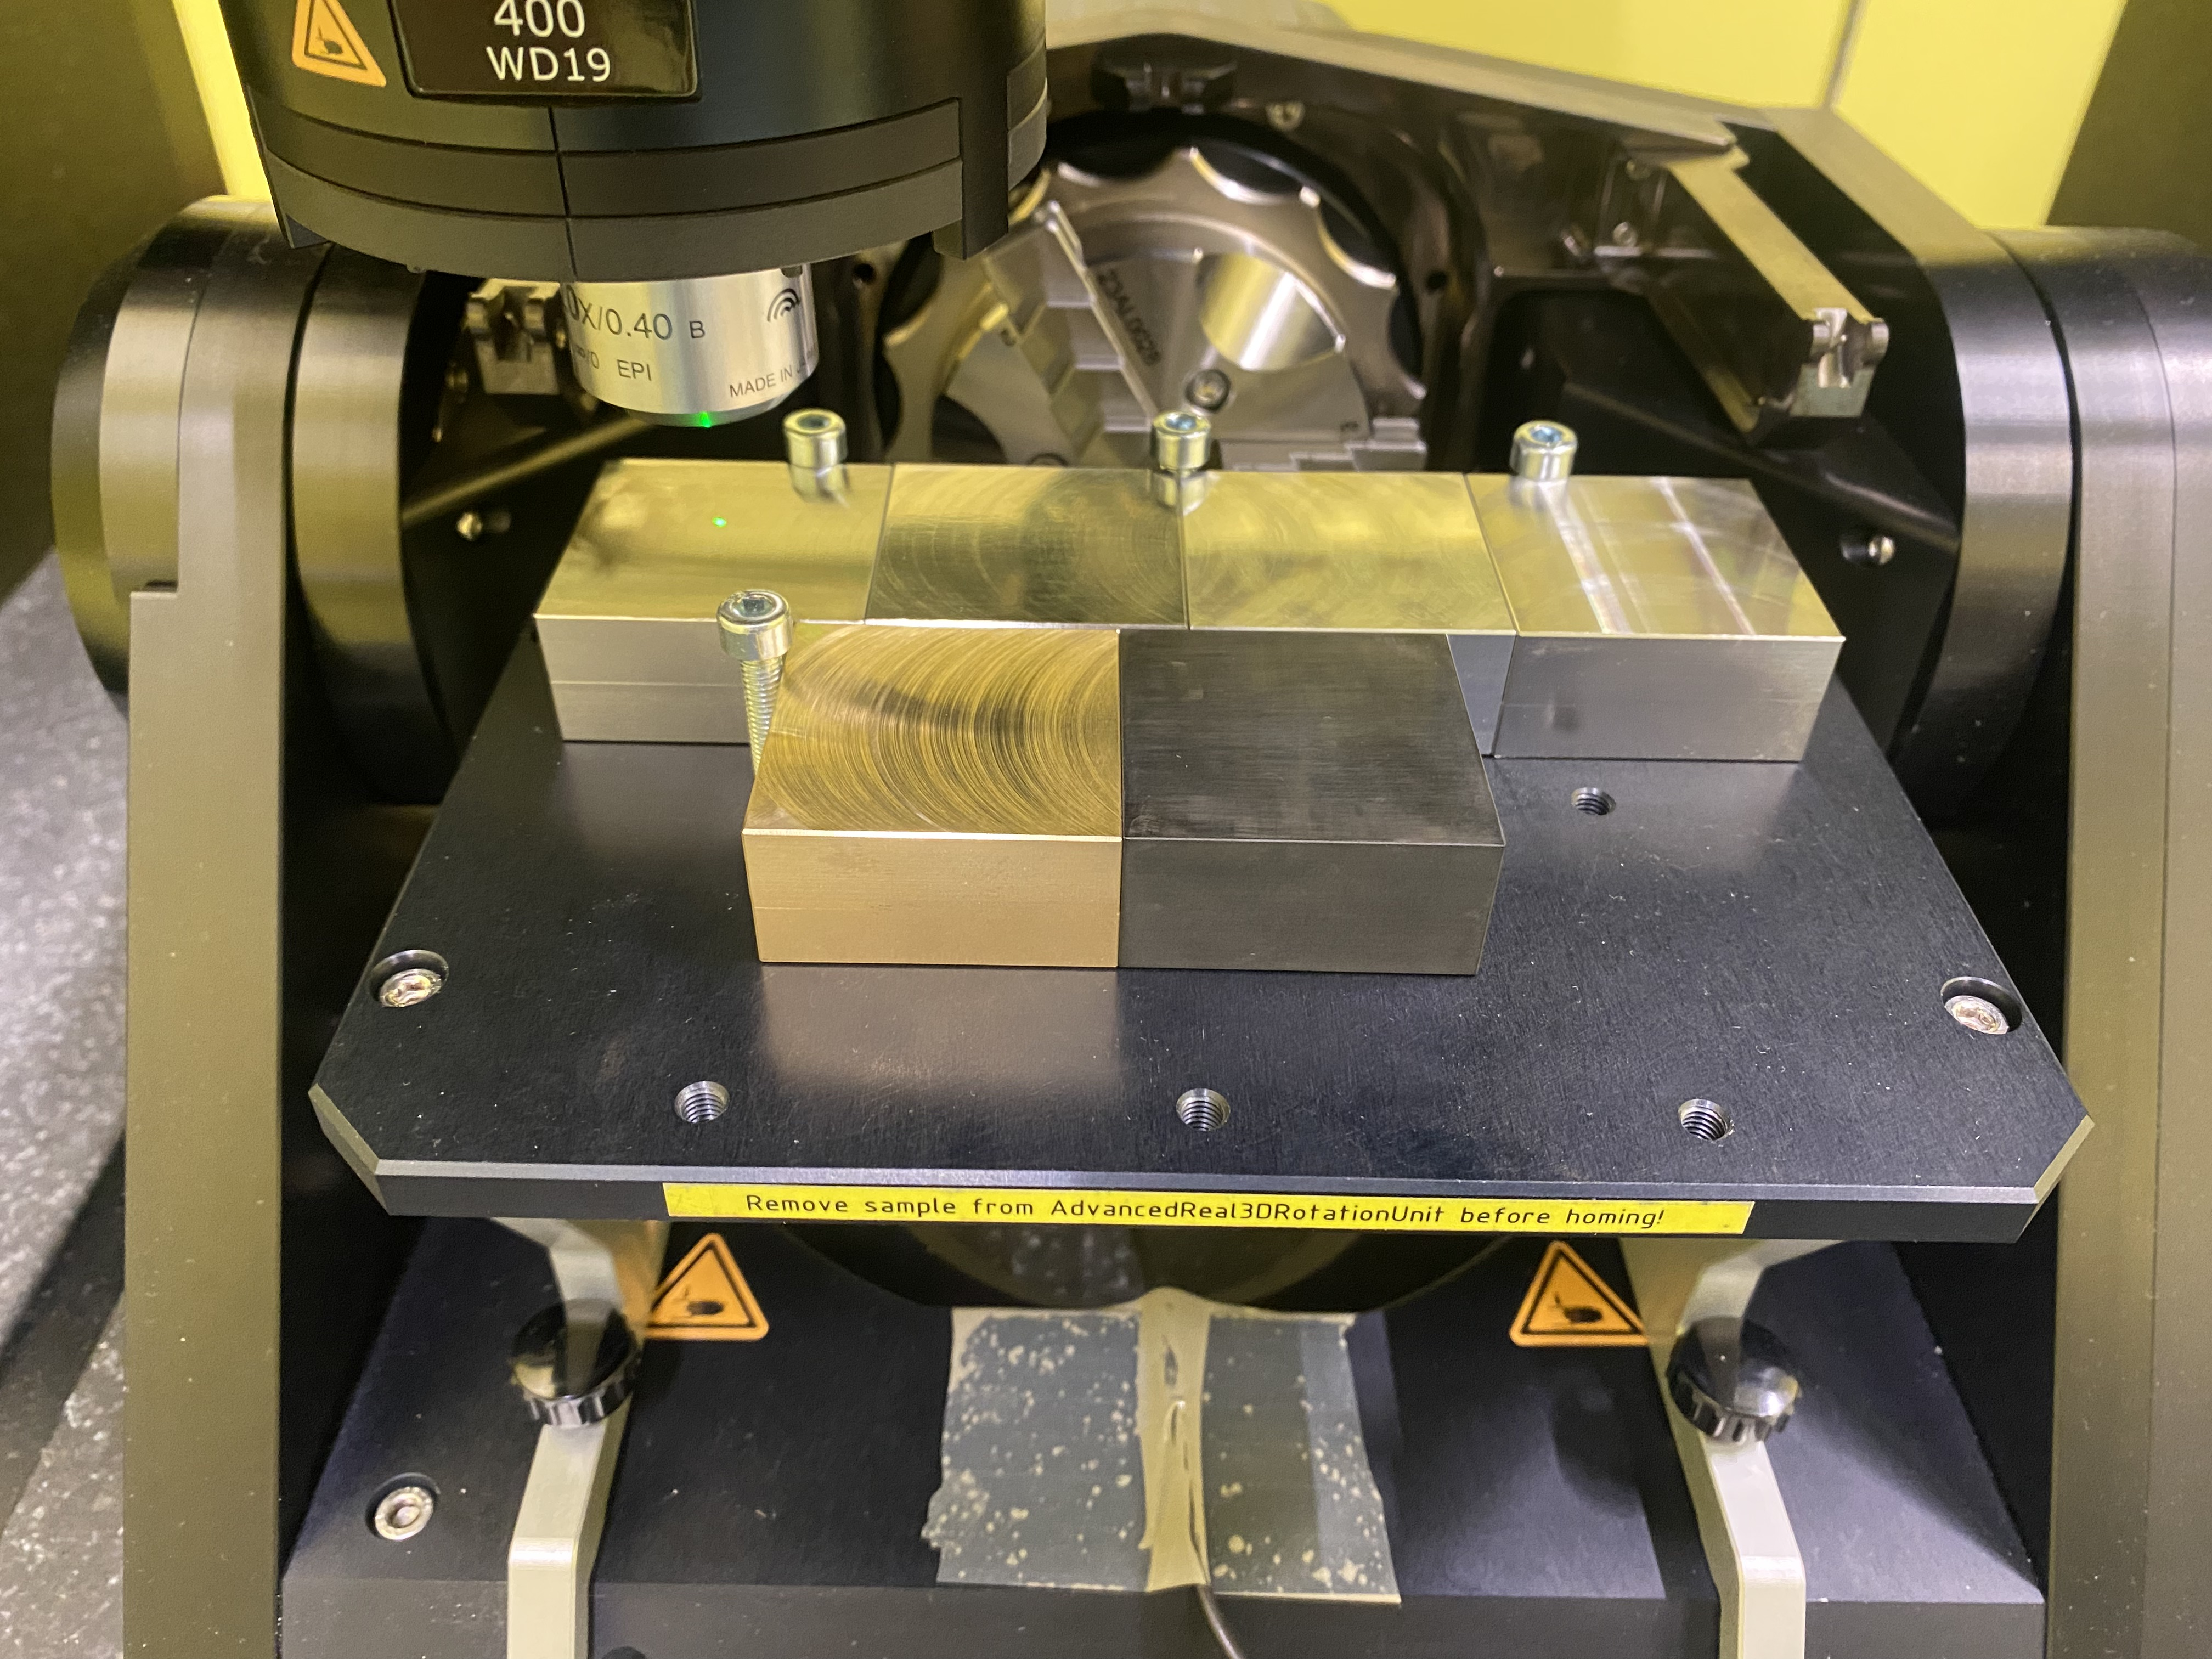
\includegraphics[width=0.62\textwidth]{IMG_6725.jpeg}
\caption{Example sample holder used during FV data collection. The holder contains representative $40\times 40\times 20$~mm specimens from the set analysed in this work. Each exposed face was measured by FV microscopy and exported as a \texttt{.sur} topography file for subsequent simulation and benchmarking.}
\label{fig:fv_holder}
\end{figure}
\unskip

A representative measured ground-truth surface is saved as both a 2D height map and a 3D rendering (Figure~\ref{fig:surface}). In other words, the FV measurement is not compared to another independent optical measurement here; rather, it provides the reference surface from which simulated classical and coincidence-proxy interferometric observations are generated.

\begin{figure}[t]
\centering
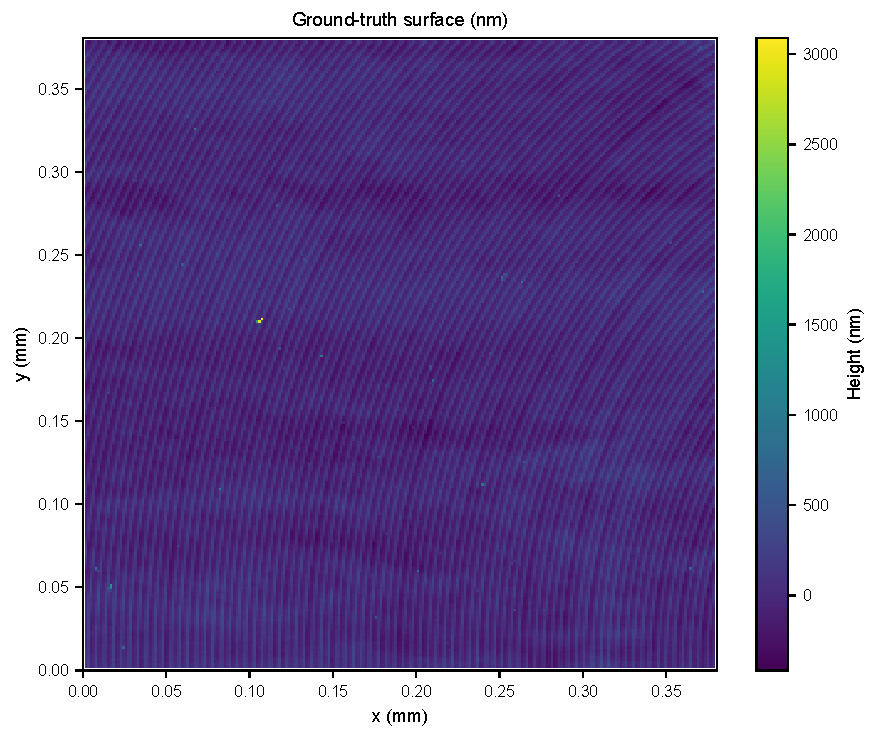
\includegraphics[width=0.48\textwidth]{paper_alicona_example/surface_true_map.pdf}\hfill
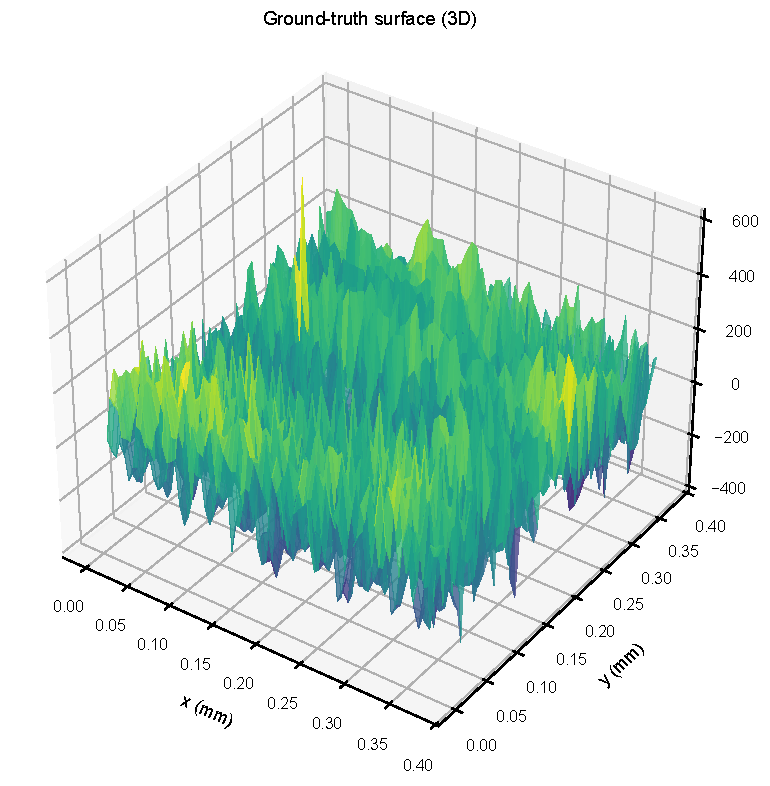
\includegraphics[width=0.48\textwidth]{paper_alicona_example/surface_true_3d.pdf}
\caption{Representative \emph{measured} benchmark surface derived from focus-variation (FV) microscopy. The sample shown is Titanium Ti-6Al-4V after turning (finishing). The displayed map is the area-averaged downsampled interferometric input surface used for the simulated classical and coincidence-proxy measurements (2D height map and 3D rendering), whereas the main reference roughness parameters are still computed on the native-resolution FV grid.}
\label{fig:surface}
\end{figure}
\unskip

\subsection{Classical interferometer: Michelson-type 4-step PSI}
A Michelson-type reflective interferometer operated in standard four-step PSI is modelled. The per-pixel intensity at phase step $d_k$ is modelled as

\begin{linenomath}
\begin{equation}
I_k = B + A\left(1 + V\cos(\phi + d_k)\right),
\end{equation}
\end{linenomath}
where $B$ is background, $A$ is amplitude, $V$ is fringe visibility, and the reflection phase is $\phi=\tfrac{4\pi}{\lambda}h(x,y)$. Shot noise is modelled by Poisson counting with a nominal photon budget (photons per pixel per frame).
Unless stated otherwise, the tables use $\lambda=532\,\mathrm{nm}$, baseline visibility $V=0.85$, and a nominal detected budget of $8\times 10^4$ photons/pixel/frame before any sample-dependent scaling; the phase-step error and drift knobs are set to zero ($\sigma_{d}=0$, no background/amplitude drift).

\subsection{Coincidence-proxy channel: coincidence PSI}
A coincidence-like observable is simulated in a four-step phase-stepped protocol such that the same phase estimator as in classical PSI can be used. The coincidence mean is modelled analogously, but with an effective wavelength determined by the reported coincidence proxy (difference synthetic wavelength or NOON-like half-wavelength), following the general synthetic-wavelength and multiphoton-phase logic used in classical two-colour and quantum interferometric sensing \cite{Zhang2022,Kotsiuba2018207,Kapale2007,Jha2011,Sharma2022}.

In this study, the coincidence channel is used as an architecture-level proxy rather than as a fully calibrated fourth-order interference transfer model. The comparison therefore asks how a coincidence-derived long-effective-wavelength observable changes reconstruction performance under matched detected-count assumptions, especially when used directly versus as a coarse prior in a hybrid pipeline.

Throughout the Results and Discussion, the label ``quantum-like'' refers only to this coincidence-proxy branch. It does not denote standalone experimental validation of entanglement-enhanced surface metrology.

Two detector models are used in this work: (i) a simple Poisson model around a cosine mean and (ii) a rate-based coincidence model with accidentals parameterised by a coincidence window and gate time. The latter is used only in the targeted detector-side sensitivity check, where a simple nonparalyzable deadtime proxy is also added.
Unless stated otherwise, the tables use $\lambda_1=810\,\mathrm{nm}$ and $\lambda_2=809\,\mathrm{nm}$, baseline visibility $V=0.6$, a nominal detected budget of $3\times 10^4$ pairs/pixel/frame before any sample-dependent scaling, and the simple (Poisson) coincidence model.

Within the present cosine--Poisson proxy, the local height-noise scale obeys the same qualitative dependence as standard PSI, namely $\sigma_h\propto \lambda_\mathrm{eff}/(4\pi V\sqrt{N})$ for detected count budget $N$. The ``matched budget'' comparison in this paper should therefore be read as a matched detected-count comparison under fixed transfer models, not as a claim of universal Fisher-equivalent normalisation across all interferometer architectures. The classical two-colour and wavelength-spacing controls are included to test whether the main regime split is robust to that resource-accounting choice.
Accordingly, a targeted budget-normalisation sensitivity control later repeats the representative NOON-like step-free case under three conventions: the paper-default budget split, equal nominal quanta per pixel, and matched detected counts in the coincidence proxy.

\subsection{Optical layouts}
Schematic optical layouts for the classical Michelson PSI and the coincidence-proxy interferometer are shown in Figure~\ref{fig:layouts}. The classical branch uses a standard reflective Michelson geometry with phase stepping in one arm, whereas the coincidence branch replaces the single intensity readout with two detector channels and coincidence logic. The purpose of Figure~\ref{fig:layouts} is therefore to make clear which parts of the benchmark differ only in the detection architecture and effective wavelength model, and which parts remain common between the compared pipelines.

\begin{figure}[t]
\centering
% TikZ optical layout schematics (not to scale)
\begin{tikzpicture}[x=0.95cm,y=0.95cm, font=\small, >=Stealth]
  \tikzset{
    beam/.style={line width=0.9pt},
    midarrow/.style={
      decoration={markings,
      mark=at position 0.55 with {\arrow{Stealth[length=2.2mm,width=1.6mm]}}},
      postaction={decorate}
    },
    fwd/.style={beam,midarrow},
    ret/.style={beam,densely dashed,midarrow},
    comp/.style={draw,fill=gray!12,rounded corners=1pt},
    detector/.style={draw,fill=gray!10,rounded corners=1pt,
                     minimum width=11mm,minimum height=6mm},
    label/.style={font=\scriptsize,fill=white,inner sep=1pt}
  }

  % ---- Beamsplitter ----
  \newcommand{\BSplate}[2]{%
    \begin{scope}
      \coordinate (bs@c) at #1;
      \draw[fill=gray!18,fill opacity=0.35,draw]
        ([shift={(-0.22,-0.22)}]bs@c) rectangle
        ([shift={(0.22,0.22)}]bs@c);
      \draw[line width=0.8pt]
        ([shift={(-0.22,-0.22)}]bs@c) --
        ([shift={(0.22,0.22)}]bs@c);
      \node[label,anchor=south west]
        at ([shift={(0.28,0.28)}]bs@c) {#2};
    \end{scope}
  }

  % ---- Mirror ----
  \newcommand{\Mir}[3]{%
    \begin{scope}
      \coordinate (m@c) at #1;
      \draw[line width=1.1pt,
            rotate around={#3:(m@c)}]
        ([shift={(-0.23,0)}]m@c) --
        ([shift={(0.23,0)}]m@c);
      \node[label,anchor=south west]
        at ([shift={(0.25,0.15)}]m@c) {#2};
    \end{scope}
  }

  % ---- Rough sample ----
  \newcommand{\SampleMirror}[3]{%
    \begin{scope}
      \coordinate (s@c) at #1;
      \draw[line width=1.1pt,
            rotate around={#3:(s@c)}]
        ([shift={(-0.23,0)}]s@c) --
        ([shift={(0.23,0)}]s@c);
      \draw[rotate around={#3:(s@c)},
            decorate,
            decoration={random steps,
            segment length=2pt,amplitude=1pt}]
        ([shift={(-0.23,0.06)}]s@c) --
        ([shift={(0.23,0.06)}]s@c);
      \node[label,anchor=south west]
        at ([shift={(0.28,0.18)}]s@c) {#2};
    \end{scope}
  }

  % ===================== (a) =====================
  \begin{scope}
    \node[anchor=north west] at (0,4.6) {\textbf{(a)}};

    \coordinate (BS)   at (2.4,2.0);
    \coordinate (Mref) at (5.4,2.0);
    \coordinate (Samp) at (2.4,3.5);
    \coordinate (Cam)  at (2.4,0.5);

    % Laser
    \draw[comp] (0.0,1.65) rectangle (1.2,2.35);
    \node[label,anchor=center] at (0.6,2.0) {Laser};
    \draw[fwd] (1.2,2.0) -- (BS);

    % BS
    \BSplate{(BS)}{BS}

    % Arms
    \draw[fwd] (BS) -- (Mref);
    \draw[fwd] (BS) -- (Samp);

    % Reference mirror + PZT
    \coordinate (mr) at (5.4,2.0);
    \draw[line width=1.1pt]
      ([yshift=-0.3cm]mr) -- ([yshift=0.3cm]mr);
    \draw[fill=gray!30]
      ([yshift=-0.25cm]mr) --
      ([shift={(0.3,0)}]mr) |-
      ([yshift=0.25cm]mr) -- cycle;
    \node[label,anchor=west] at (5.9,2.0) {PZT};

    % Sample
    \coordinate (sampC) at (2.4,3.5);
    \draw[line width=1.1pt]
      ([xshift=-0.3cm]sampC) -- ([xshift=0.3cm]sampC);
    \draw[decorate,
          decoration={random steps,
          segment length=2pt,amplitude=1pt}]
      ([xshift=-0.3cm,yshift=-0.01cm]sampC) --
      ([xshift=0.3cm,yshift=-0.01cm]sampC);
    \node[label,anchor=center] at (2.4,3.5) {Sample};

    % Return
    \draw[ret] ([yshift=0.08cm]Mref) -- ([yshift=0.08cm]BS);
    \draw[ret] ([xshift=0.08cm]Samp) -- ([xshift=0.08cm]BS);

    % Lens + camera
    \coordinate (LensC) at (2.4,1.25);
    \draw[line width=0.9pt] (2.4,1.25) ellipse (0.35 and 0.08);
    \draw[fwd] (BS) -- (LensC);
    \draw[fwd] (LensC) -- (Cam);

    \draw[detector] (1.8,0.2) rectangle (3.0,0.8);
    \node at (2.4,0.5) {Camera};
  \end{scope}

  % ===================== (b) =====================
  \begin{scope}[shift={(0,-6.5)}]
    \node[anchor=north west] at (0,5.2) {\textbf{(b)}};

    \coordinate (BS1) at (1.8,1.5);
    \coordinate (Mtop) at (1.8,3.5);
    \coordinate (Sbot) at (6.0,1.5);
    \coordinate (BS2) at (6.0,3.5);

    % Source
    \draw[comp] (0.0,1.15) rectangle (1.20,1.85);
    \node[label,anchor=center] at (0.6,1.5) {SPDC};
    \draw[fwd] (1.2,1.5) -- (BS1);

    % BS1
    \BSplate{(BS1)}{BS}

    % Top arm
    \draw[fwd] (BS1) -- (Mtop);
    \Mir{(Mtop)}{M}{45}

    \coordinate (PSin) at (3.6,3.5);
    \coordinate (PSout) at (4.4,3.5);
    \draw[fwd] (Mtop) -- (PSin);
    \draw[fwd] (PSout) -- (BS2);

    \draw[comp,fill=white]
      (3.6,3.3) rectangle (4.4,3.7);
    \node[label,anchor=center] at (4.0,3.5) {PS};

    % Bottom arm
    \draw[fwd] (BS1) -- (Sbot);
    \SampleMirror{(Sbot)}{Sample}{45}
    \draw[fwd] (Sbot) -- (BS2);

    % BS2
    \BSplate{(BS2)}{BS}

    % Outputs
    \coordinate (D1) at (7.8,3.5);
    \coordinate (D2) at (6.0,5.0);

    \draw[fwd] (BS2) -- (D1);
    \draw[fwd] (BS2) -- (D2);

    \draw[detector] (7.4,3.2) rectangle (8.2,3.8);
    \node at (7.8,3.5) {$D_1$};

    \draw[detector] (5.6,4.7) rectangle (6.4,5.3);
    \node at (6.0,5.0) {$D_2$};

    \draw[comp] (7.4,4.7) rectangle (8.6,5.3);
    \node at (8.0,5.0) {Coinc.};

    \draw[beam] (7.8,3.8) -- (7.8,4.7);
    \draw[beam] (6.4,5.0) -- (7.4,5.0);

    \draw[->,beam] (8.6,5.0) -- (9.4,5.0);
    \node[label,anchor=west] at (9.5,5.0) {$G^{(2)}$};
  \end{scope}
\end{tikzpicture}

\caption{Schematic optical layouts used for method description. (a) Classical Michelson-type 4-step PSI. (b) Coincidence-proxy interferometer with two detection channels and coincidence logic. Legend: BS/BS1/BS2, beam splitter; M, mirror; Sample, reflective test surface; PS, phase shifter; D1 and D2, single-photon detectors; ``Coincidence'', correlator producing $G^{(2)}$. Straight lines show beam paths; arrows indicate nominal propagation direction; dashed segments denote the return path in the reflective geometry.}
\label{fig:layouts}
\end{figure}
\unskip

\subsection{Reconstruction and metrics}
Wrapped phase is reconstructed by a standard 4-step PSI estimator (or least-squares variant), unwrapped in the main benchmark by a simple separable 2D scheme (rows then columns), and converted to height via $h=\tfrac{\lambda}{4\pi}\phi$. Because direct branches could in principle be sensitive to that unwrap path, a targeted control later reruns the measured-surface benchmark with a global least-squares Poisson unwrap; that control is reported in the Results section rather than used to redefine the main paper workflow.

For the hybrid reconstruction, the final height map is not obtained by averaging the classical and coincidence-based reconstructions. Instead, a coarse-to-fine unwrapping strategy is used. First, a coarse absolute-height estimate $h_\mathrm{coarse}(x,y)$ is reconstructed from the coincidence-based channel using its effective wavelength. Second, the classical PSI branch provides the wrapped short-wavelength phase $\phi_{\mathrm{short},w}(x,y)$, from which the principal-value short-wavelength height
\begin{linenomath}
\begin{equation}
h_0(x,y)=\frac{\lambda_\mathrm{short}}{4\pi}\,\phi_{\mathrm{short},w}(x,y)
\end{equation}
\end{linenomath}
is computed. Because adding $2\pi$ to phase in reflective geometry corresponds to adding $\lambda_\mathrm{short}/2$ in height, the hybrid estimator chooses the integer fringe order $k(x,y)$ that makes the short-wavelength reconstruction closest to the coarse prior,
\begin{linenomath}
\begin{equation}
k(x,y)=\mathrm{round}\!\left(\frac{h_\mathrm{coarse}(x,y)-h_0(x,y)}{\lambda_\mathrm{short}/2}\right),
\end{equation}
\end{linenomath}
and the final hybrid height is then
\begin{linenomath}
\begin{equation}
h_\mathrm{hyb}(x,y)=h_0(x,y)+k(x,y)\frac{\lambda_\mathrm{short}}{2}.
\end{equation}
\end{linenomath}
Thus, the coincidence-based channel supplies only a coarse absolute-height prior for fringe-order selection, while the fine texture in the final hybrid map is still carried by the short-wavelength classical PSI branch. When the paper refers to H-diff, H-noon2, or related labels, the suffix indicates which coincidence-proxy channel supplied $h_\mathrm{coarse}$.

An auxiliary classical two-colour control is also used later in the Results section. In that control, the coincidence-derived coarse prior is replaced by a classical synthetic-wavelength prior reconstructed from two classical PSI stacks at 810 and 809~nm, allowing generic two-wavelength behaviour to be separated from coincidence-model effects.

The following are reported:
\begin{itemize}
\item height RMSE after plane detrending (texture-focused),
\item roughness biases for Sa, Sq, and Sz, where the main benchmark uses reference values computed directly from the native FV \texttt{.sur} height map and an added matched-bandwidth control recomputes the same biases against the area-averaged benchmark grid used by the forward model.
\end{itemize}

These areal descriptors are chosen because both the FV reference and the interferometric reconstructions are full-field topography maps rather than extracted line profiles. $S_a$ tracks mean texture amplitude, $S_q$ is the RMS height descriptor and therefore the natural bridge to the synthetic-sweep roughness parameter, and $S_z$ tracks extreme envelope excursions. Profile quantities such as $R_a$ or $R_q$ are not used as primary endpoints here because they would require an additional line-selection convention that is orthogonal to the architectural comparison. $S_z$ is nevertheless retained because long-wavelength channels may follow broad peak-to-valley structure, but it is interpreted as the least stable endpoint and is never treated in isolation as proof of overall metrology superiority.

\subsection{Reproducibility and canonical workflow}
To minimise hidden manual processing, the manuscript uses fixed reproducibility workflows rather than ad hoc commands. The main measured-surface artefacts are regenerated by \path{scripts/run_paper_measured_benchmark.py}, which reruns the FV benchmark, refreshes the manuscript figures, and rewrites the tables derived from the benchmark outputs and SUR headers. Targeted measured-surface controls are regenerated by \path{scripts/run_paper_resolution_sensitivity.py}, \path{scripts/run_paper_unwrap_control.py}, \path{scripts/run_paper_classical_two_color_control.py}, and \path{scripts/run_paper_measured_rate_control.py}. The step-free optical-property sweep is regenerated by \path{scripts/run_paper_optprops.py}, while the step/ambiguity, non-ideal stress, and detector-sensitivity controls are produced by \path{scripts/run_paper_step_regime_control.py}, \path{scripts/make_nonideal_stress_artifacts.py}, and \path{scripts/run_paper_detector_sensitivity.py}.

Manuscript-ready tables are written into \path{manuscript/tables}, the paper is compiled from \path{manuscript/main.tex} with \path{latexmk -pdf -bibtex -interaction=nonstopmode main.tex}, and the exact submission snapshot is indexed in \path{docs/submission_snapshot_manifest.md}. The repository also contains smoke runs, exploratory sweeps, and intermediate plots used during development; those files are excluded from the submission record.

%%%%%%%%%%%%%%%%%%%%%%%%%%%%%%%%%%%%%%%%%%
\section{Results}
\subsection{Benchmark on focus-variation measured surfaces}
To align the evaluation with realistic textures, the classical, quantum-like, and hybrid pipelines are benchmarked on $n=59$ measured surfaces acquired using focus-variation (FV) microscopy and exported as Mountains/DigitalSurf \texttt{.sur} height maps. The dataset spans six material groups and ten treatment classes, and Table~\ref{tab:measured_surface_metadata} summarises the corresponding SUR-header grid, field-of-view, and sampling ranges. For each sample, the main reference roughness parameters are computed directly on the native FV \texttt{.sur} grid after masking only explicit invalid pixels and removing a best-fit plane, whereas the interferometric forward model uses a separate area-averaged downsampled simulation surface derived from the same measurement. Simulated classical intensity frames and simulated coincidence-like measurements are then generated from that common simulation surface and reconstructed for comparison. The canonical paper benchmark now uses repeated stochastic realisations per surface and method, which are collapsed to surface-level medians before between-surface statistics are reported. Filenames encode material and surface-treatment codes which are decoded into consistent English labels for reporting; results are summarised by grouping across materials (Table~\ref{tab:alicona_rmse_by_material}) and across surface treatments (Table~\ref{tab:alicona_rmse_by_treatment}) using robust per-surface medians with interquartile ranges rather than mean $\pm$ std summaries.

The overall measured-surface height-error behaviour is summarised in Figure~\ref{fig:alicona_rmse_summary}. The left panel condenses the detrended RMSE distributions across all measured samples, while the right panel shows how those RMSE values evolve with the roughness level of the FV reference surfaces. The figure provides the first high-level view of the regime split developed later in the section: the hybrid branch remains the strongest overall height-fidelity option, while the direct coincidence-like branch and the classical baseline trade wins only in narrower subsets of the dataset.

% Auto-generated by scripts/make_table_from_sur_benchmark.py
\begin{table}[H]
\centering
\footnotesize
\setlength{\tabcolsep}{2.8pt}
\caption{Height RMSE (after plane detrending) grouped by material. Entries report the median surface-level RMSE with the first and third quartiles in brackets after collapsing repeated runs within each measured surface and method.}
\label{tab:alicona_rmse_by_material}
\resizebox{\textwidth}{!}{%
\begin{tabular}{lrccc}
\toprule
Material & n & Classical & Coincidence-proxy & Hybrid \\
\midrule
Aluminium 7075 & 10 & $829.4$ [$197.1$, $2775.4$] & $709.7$ [$709.4$, $710.7$] & $234.3$ [$159.8$, $1115.3$] \\
Brass & 10 & $1560.2$ [$664.3$, $2476.8$] & $710.4$ [$709.3$, $710.7$] & $731.5$ [$229.6$, $1701.6$] \\
Graphite & 9 & $1754.1$ [$771.0$, $2038.7$] & $709.4$ [$709.0$, $709.8$] & $1144.0$ [$259.6$, $1411.2$] \\
Stainless steel 1.4301 (AISI 304) & 10 & $1028.0$ [$505.0$, $1090.1$] & $709.7$ [$709.2$, $710.3$] & $273.8$ [$268.0$, $365.0$] \\
Steel C45 & 10 & $1017.1$ [$776.4$, $4827.9$] & $709.4$ [$708.7$, $710.8$] & $340.9$ [$249.7$, $2463.3$] \\
Titanium & 10 & $947.1$ [$902.6$, $1157.7$] & $709.4$ [$708.4$, $709.9$] & $260.9$ [$204.7$, $402.1$] \\
\bottomrule
\end{tabular}
}%
\end{table}

% Auto-generated by scripts/make_table_from_sur_benchmark.py
\begin{table}[H]
\centering
\footnotesize
\setlength{\tabcolsep}{2.8pt}
\caption{Height RMSE (after plane detrending) grouped by treatment class. Entries report the median surface-level RMSE with the first and third quartiles in brackets after collapsing repeated runs within each measured surface and method.}
\label{tab:alicona_rmse_by_treatment}
\resizebox{\textwidth}{!}{%
\begin{tabular}{lrccc}
\toprule
Treatment & n & Classical & Coincidence-proxy & Hybrid \\
\midrule
Grinding & 6 & $872.7$ [$211.9$, $1223.3$] & $710.4$ [$709.8$, $710.8$] & $211.9$ [$161.2$, $388.3$] \\
Honed & 6 & $771.3$ [$708.0$, $972.5$] & $709.2$ [$709.0$, $710.0$] & $266.7$ [$259.0$, $381.3$] \\
Glass bead blasted & 6 & $952.1$ [$898.9$, $2196.9$] & $708.4$ [$708.0$, $709.4$] & $305.1$ [$226.6$, $1587.3$] \\
Burnishing & 5 & $349.9$ [$161.4$, $752.8$] & $709.9$ [$709.0$, $711.1$] & $267.2$ [$154.6$, $286.3$] \\
Turning (roughing) & 6 & $3434.2$ [$2611.2$, $6257.8$] & $709.4$ [$708.7$, $710.4$] & $1387.3$ [$1110.0$, $1764.8$] \\
Turning (finishing) & 6 & $1150.2$ [$755.3$, $1830.5$] & $709.1$ [$708.8$, $709.3$] & $483.1$ [$211.2$, $1228.1$] \\
Milling (roughing) & 6 & $685.0$ [$76.2$, $1156.5$] & $709.8$ [$709.6$, $710.2$] & $224.8$ [$159.2$, $303.9$] \\
Milling (finishing) & 6 & $1043.5$ [$648.0$, $1134.0$] & $709.7$ [$709.5$, $710.2$] & $236.8$ [$172.4$, $391.2$] \\
Wire EDM (roughing) & 6 & $4867.5$ [$2550.8$, $5594.0$] & $710.0$ [$709.1$, $711.8$] & $3318.1$ [$1691.3$, $3444.1$] \\
Wire EDM (finishing) & 6 & $1089.9$ [$990.8$, $1590.2$] & $709.9$ [$709.2$, $710.8$] & $401.8$ [$244.1$, $966.1$] \\
\bottomrule
\end{tabular}
}%
\end{table}


Those robust grouped summaries sharpen the regime split. Hybrid gives the lowest median material-wise height RMSE for Aluminium 7075, stainless steel 1.4301, steel C45, and titanium, whereas the direct quantum-like branch is the grouped median winner only for brass and graphite. Across treatments, hybrid gives the lowest median height RMSE in eight of ten classes; the only grouped exceptions are turning (roughing) and wire-EDM (roughing), where the direct quantum-like branch is still preferred. Classical PSI is therefore an essential short-wavelength reference and the donor branch inside the hybrid estimator, but it is not the robust median winner in any grouped measured-surface slice.

\begin{figure}[t]
\centering
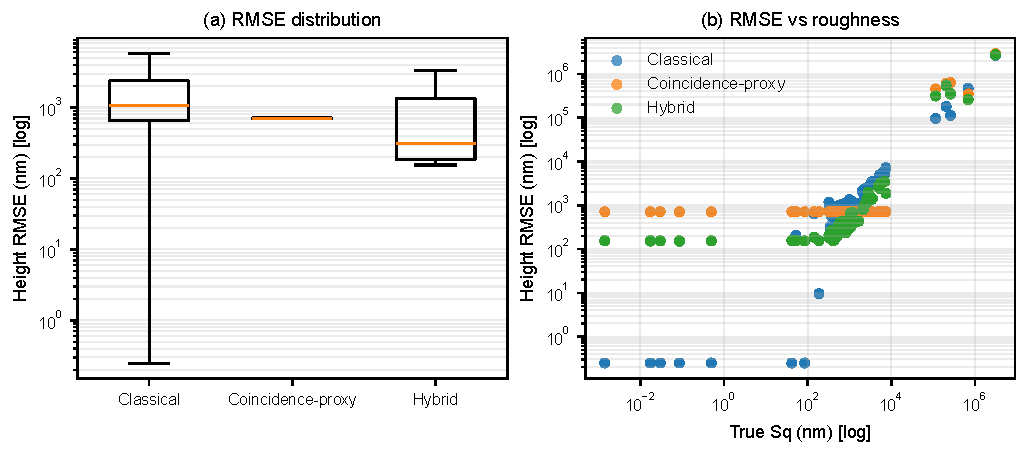
\includegraphics[width=0.92\textwidth]{paper_alicona_benchmark/figures/rmse_measured_summary.pdf}
\caption{Measured-surface benchmark summary across all FV \texttt{.sur} samples: height RMSE distributions by method and RMSE trends vs surface roughness. All values are computed from the measured height maps (after plane detrending).}
\label{fig:alicona_rmse_summary}
\end{figure}
\unskip

Because the metrology target is not only the recovered height map but also the derived areal texture descriptors, the same FV benchmark was further compared directly in terms of the reconstructed roughness parameters. Figure~\ref{fig:alicona_roughness_summary} plots estimated Sa, Sq, and Sz against the corresponding native-resolution reference values computed directly from the FV \texttt{.sur} height maps after explicit-invalid masking and plane detrending. Using that stricter native-grid reference still matters: the FV data retain more local variance and more extreme peak-to-valley excursions than the downsampled simulation surface used by the interferometric forward model. As a result, Sq and especially Sz remain more sensitive than Sa to missing high-amplitude content. Under this native-grid criterion, the hybrid branch is the most consistently texture-faithful for Sa, whereas the quantum-like branch is only selectively favoured for Sq and, more strongly but less stably, for Sz.

For the remainder of the measured-surface section, detrended height RMSE is treated as the primary endpoint because it is the only ranking that remains materially stable across grouped slices and stronger classical controls. The roughness descriptors are therefore reported as secondary diagnostics of bandwidth retention and envelope following rather than as independent evidence of a universally preferred workflow.

Secondary roughness diagnostics nevertheless explain how the branches fail. Figure~\ref{fig:alicona_roughness_summary} plots estimated Sa, Sq, and Sz against the corresponding native-resolution reference values computed directly from the FV \texttt{.sur} height maps after explicit-invalid masking and plane detrending. This native-grid comparison is intentionally stricter than the benchmark grid used in the forward model, but it should not be treated in isolation because the FV reference retains more local variance and more extreme peak-to-valley excursions than the downsampled simulation surface. Under this native-grid view, the hybrid branch remains closest for Sa, whereas the direct coincidence-proxy branch is selectively favoured for Sq and especially Sz.

That native-grid ranking is not the main workflow recommendation. Table~\ref{tab:alicona_roughness_median_abs} reports the native-grid medians, while Table~\ref{tab:alicona_roughness_median_abs_bw} recomputes the same roughness errors against the area-averaged benchmark grid used by the interferometric forward model. Under that matched-bandwidth control, the hybrid branch remains best for Sa and takes over Sq, whereas the direct coincidence-proxy branch remains best only for Sz. The apparent native-grid Sq advantage of the direct branch is therefore largely explained by the native-grid versus benchmark-grid bandwidth mismatch. The remaining Sz advantage is narrower and should be read as envelope following rather than as reliable texture recovery, particularly because the best native-grid $|\Delta S_z|$ branch still exceeds the descriptor-scaled tolerance band on 74.6\% of surfaces (Table~\ref{tab:benchmark_tolerance_rates}).

% Auto-generated by scripts/make_table_from_sur_roughness.py
\begin{table}[H]
\centering
\footnotesize
\caption{Native-grid diagnostic stress test for the measured-surface benchmark: median absolute roughness-parameter error relative to roughness values computed on the native FV \texttt{.sur} height maps after masking explicit invalid pixels and removing a best-fit plane. This comparison is intentionally stricter than the forward-model bandwidth and is retained as a reference-sensitivity diagnostic rather than as the primary roughness ranking.}
\label{tab:alicona_roughness_median_abs}
\begin{tabular}{lrrr}
\toprule
Method & Median $|\Delta S_a|$ (nm) & Median $|\Delta S_q|$ (nm) & Median $|\Delta S_z|$ (nm) \\
\midrule
Classical & $302.2$ & $423.4$ & $37163.2$ \\
Coincidence-proxy & $308.1$ & $397.0$ & $25745.5$ \\
Hybrid & $129.6$ & $419.1$ & $37528.3$ \\
\bottomrule
\end{tabular}
\end{table}

% Auto-generated by scripts/make_table_from_sur_roughness.py
\begin{table}[H]
\centering
\footnotesize
\caption{Matched-bandwidth control for the measured-surface benchmark: median absolute roughness-parameter error relative to roughness values computed on the same area-averaged benchmark grid used by the interferometric forward model.}
\label{tab:alicona_roughness_median_abs_bw}
\begin{tabular}{lrrr}
\toprule
Method & Median $|\Delta S_a|$ (nm) & Median $|\Delta S_q|$ (nm) & Median $|\Delta S_z|$ (nm) \\
\midrule
Classical & $337.9$ & $435.8$ & $8465.9$ \\
Coincidence-proxy & $333.5$ & $396.2$ & $2653.1$ \\
Hybrid & $86.3$ & $152.4$ & $5349.5$ \\
\bottomrule
\end{tabular}
\end{table}


\begin{figure}[t]
\centering
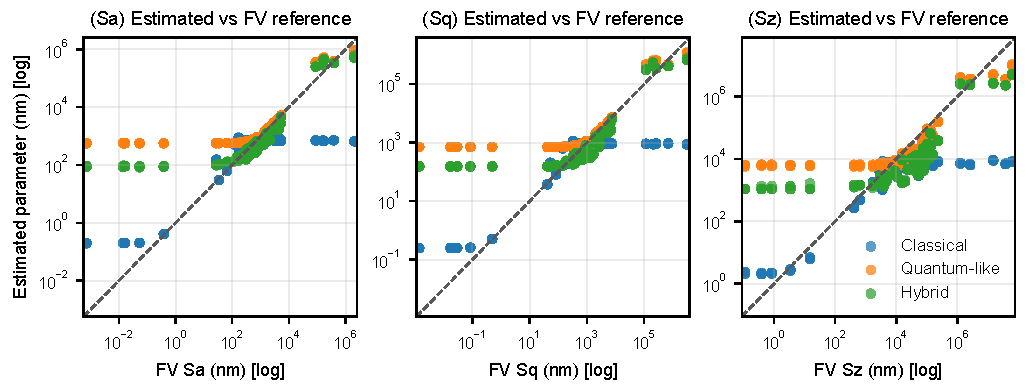
\includegraphics[width=0.98\textwidth]{paper_alicona_benchmark/figures/roughness_measured_summary.pdf}
\caption{Direct comparison of areal roughness parameters estimated from the simulated interferometric reconstructions against the corresponding values computed from the Alicona reference height maps. Each point is one measured \texttt{.sur} surface; the dashed line marks perfect agreement. This native-grid view is diagnostic rather than definitive for workflow selection because the interferometric forward model operates on the downsampled benchmark grid. The hybrid branch remains strongest for Sa, whereas the direct coincidence-proxy branch more often follows the native-grid Sq and Sz values because it retains broad-envelope excursions more readily than fine texture.}
\label{fig:alicona_roughness_summary}
\end{figure}
\unskip

The residual/Bland--Altman-style view in Figure~\ref{fig:alicona_roughness_bias} makes the bias structure explicit. For Sa and Sq, the direct quantum-like branch is generally shifted upward relative to the native-grid FV reference, whereas the hybrid branch stays closer to zero across the central mass of surfaces. For Sz, all three branches remain negatively biased relative to the native-grid FV reference, but the central tendency is least negative for the quantum-like branch. The broad spread across all three panels confirms that the bias structure is heteroscedastic rather than a single global offset.

\begin{figure}[t]
\centering
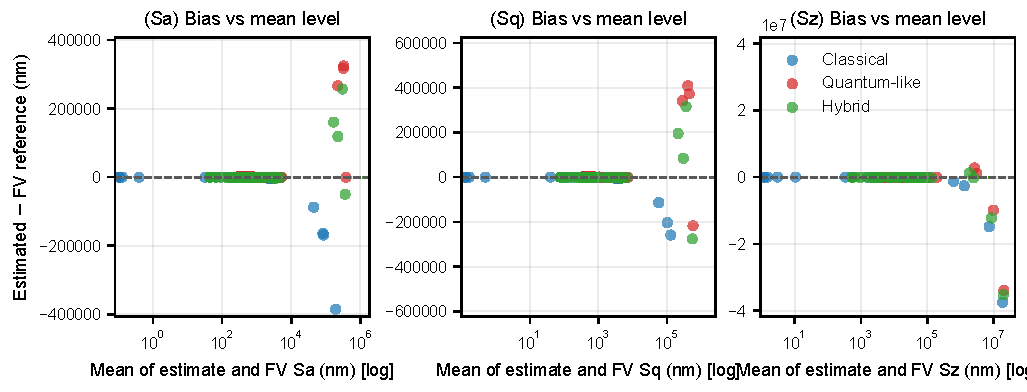
\includegraphics[width=0.98\textwidth]{paper_alicona_benchmark/figures/roughness_measured_bland_altman.pdf}
\caption{Bland--Altman-style residual view for the measured-surface roughness benchmark. The horizontal dashed line marks zero bias, while dotted lines mark the method-wise median bias in each panel. The figure makes the endpoint split more explicit: the quantum-like branch shifts upward for Sa and Sq, while its central Sz bias remains less negative than the corresponding classical and hybrid offsets.}
\label{fig:alicona_roughness_bias}
\end{figure}
\unskip

The treatment-resolved view in Figure~\ref{fig:alicona_roughness_by_treatment} shows that this is not a uniform material-independent effect. Hybrid reconstruction keeps the smallest median $|\Delta S_a|$ and $|\Delta S_q|$ in several finishing-style classes, whereas the quantum-like branch often produces the smallest $|\Delta S_z|$ on smoother treatments such as honed, burnished, and turned-finish surfaces. On rougher classes, especially turning (roughing), milling (finishing), and wire-EDM textures, all three branches degrade sharply, confirming that the measured-surface advantage is process dependent rather than universal. The treatment-holdout analysis below shows that these roughness rankings are not stable enough to serve as a general selection rule, particularly for $S_a$ and $S_q$.

To make that regime split explicit at the per-surface level, Table~\ref{tab:dominance_summary} reports winner counts for each endpoint. The dominance view reinforces the same message as the grouped medians for height fidelity: hybrid reconstruction remains strongest overall for height RMSE (32 wins). The roughness endpoints are more split. For $|\Delta S_a|$, the winner counts are effectively tied across the three branches (20 classical, 20 quantum-like, and 19 hybrid wins), whereas the quantum-like branch dominates $|\Delta S_q|$ (26 wins) and especially $|\Delta S_z|$ (39 wins). The low-roughness column still shows that the hybrid advantage is concentrated most strongly in the smoother regime for height fidelity, while the rougher column remains selectively favourable to the quantum-like branch for envelope-dominated descriptors. These winner counts are descriptive only and should be read alongside the holdout and tolerance summaries rather than as deployable ranking rules.

% Auto-generated by scripts/make_benchmark_comparison_tables.py
\begin{table}[t]
\centering
\footnotesize
\setlength{\tabcolsep}{4pt}
\caption{Per-surface winner counts in the measured-surface benchmark. For each measured \texttt{.sur} surface, the ``winner'' is the method with the lowest height RMSE or the smallest absolute roughness bias for the stated endpoint. Roughness endpoints use the matched-bandwidth benchmark-grid reference. The low-roughness column isolates the smoother benchmark-grid group ($S_a<500$~nm), whereas the rougher column aggregates the two highest roughness bins ($S_a\geq 1000$~nm).}
\label{tab:dominance_summary}
\resizebox{\textwidth}{!}{%
\begin{tabular}{p{3.4cm}ccc ccc ccc}
\toprule
& \multicolumn{3}{c}{All measured surfaces} & \multicolumn{3}{c}{$S_a<500$~nm} & \multicolumn{3}{c}{$S_a\geq 1000$~nm}\\
Endpoint & Classical & Coincidence-proxy & Hybrid & Classical & Coincidence-proxy & Hybrid & Classical & Coincidence-proxy & Hybrid\\
\midrule
Height RMSE & 12 & 15 & 32 & 8 & 0 & 25 & 4 & 14 & 1 \\
$|\Delta S_a|$ & 19 & 17 & 23 & 12 & 0 & 21 & 3 & 16 & 0 \\
$|\Delta S_q|$ & 17 & 17 & 25 & 11 & 0 & 22 & 3 & 16 & 0 \\
$|\Delta S_z|$ & 16 & 30 & 13 & 12 & 9 & 12 & 2 & 16 & 1 \\
\bottomrule
\end{tabular}
}%
\end{table}


Bootstrap uncertainty and endpoint-referenced tolerance summaries sharpen that caution further. Table~\ref{tab:benchmark_bootstrap_ci} shows that the hybrid branch gives the smallest surface-level median height RMSE and $|\Delta S_a|$, while the quantum-like branch remains the most favourable direct branch for native-grid $|\Delta S_z|$ and only narrowly for native-grid $|\Delta S_q|$. Table~\ref{tab:benchmark_repeatability} adds the within-surface repeat-dispersion view and shows that the stochastic Monte-Carlo spread is substantially smaller than the between-surface regime split that drives the main ranking. Tables~\ref{tab:benchmark_holdout_material} and \ref{tab:benchmark_holdout_treatment} then test whether that ranking survives leave-one-group-out splits instead of being trained and praised on the same aggregate alone. For height RMSE, hybrid remains the training-set winner in all six material and all ten treatment splits, with held-out agreement on 4/6 and 8/10 splits, respectively. The roughness endpoints are less stable across treatments: $|\Delta S_a|$ drops to 50\% treatment-holdout agreement, $|\Delta S_q|$ falls to 0\%, and even the more stable native-grid $|\Delta S_z|$ ranking should still be read as process-sensitive envelope following rather than as a globally transferable roughness result. Table~\ref{tab:benchmark_tolerance_rates} makes that limitation quantitative: the descriptor-scaled tolerance band is exceeded on 74.6\% of surfaces even for the best native-grid $|\Delta S_z|$ branch, compared with 79.7\% for classical and 81.4\% for hybrid. The paired-effect summary in Table~\ref{tab:benchmark_paired_effects} makes the same trade-off more explicit: hybrid remains the dominant paired choice for height RMSE, while the quantum-like branch retains the strongest paired advantage for $|\Delta S_z|$. These effects are descriptive rather than confirmatory, but they are more informative than p-values alone about the magnitude and frequency of the regime split.

% Auto-generated by scripts/make_benchmark_stat_tables.py
\begin{table}[t]
\centering
\footnotesize
\setlength{\tabcolsep}{4pt}
\caption{Measured-surface benchmark summary using surface-level medians over $n=59$ unique measured surfaces with percentile bootstrap 95\% confidence intervals. The canonical paper benchmark uses $n_\mathrm{rep}=4$ Monte Carlo realisations per surface and method; repeated runs are collapsed within each surface before between-surface uncertainty is estimated. Roughness endpoints use the matched-bandwidth benchmark-grid reference rather than the native FV grid.}
\label{tab:benchmark_bootstrap_ci}
\resizebox{\textwidth}{!}{%
\begin{tabular}{lccc}
\toprule
Endpoint & Classical & Coincidence-proxy & Hybrid \\
\midrule
Height RMSE (nm) & $1065.7$ [$898.4$, $1205.6$] & $709.6$ [$709.4$, $709.9$] & $314.0$ [$259.6$, $435.6$] \\
$|\Delta S_a|$ (nm) & $337.9$ [$228.3$, $416.4$] & $332.5$ [$293.2$, $382.3$] & $88.4$ [$63.7$, $153.5$] \\
$|\Delta S_q|$ (nm) & $435.8$ [$278.2$, $549.6$] & $396.0$ [$327.0$, $457.8$] & $153.3$ [$104.3$, $213.9$] \\
$|\Delta S_z|$ (nm) & $8465.9$ [$4200.3$, $17111.4$] & $2509.1$ [$1926.6$, $4127.1$] & $5349.5$ [$2204.4$, $15599.6$] \\
\bottomrule
\end{tabular}
}%
\end{table}

% Auto-generated by scripts/make_benchmark_stat_tables.py
\begin{table}[t]
\centering
\footnotesize
\setlength{\tabcolsep}{4pt}
\caption{Within-surface stochastic dispersion in the measured-surface benchmark over $n=59$ unique surfaces. Entries report the median per-surface interquartile range of repeated-run errors, with first and third quartiles in brackets, using $n_\mathrm{rep}=4$ Monte Carlo realisations per surface and method. Lower values indicate better repeatability under the simulator's stochastic shot-noise model.}
\label{tab:benchmark_repeatability}
\resizebox{\textwidth}{!}{%
\begin{tabular}{lccc}
\toprule
Endpoint & Classical & Coincidence-proxy & Hybrid \\
\midrule
Height RMSE (nm) & $2.6$ [$0.7$, $3.9$] & $1.7$ [$1.3$, $3.0$] & $0.9$ [$0.5$, $1.5$] \\
$|\Delta S_a|$ (nm) & $2.7$ [$1.3$, $4.4$] & $2.1$ [$1.1$, $3.2$] & $2.2$ [$1.3$, $3.5$] \\
$|\Delta S_q|$ (nm) & $3.5$ [$1.5$, $5.8$] & $2.1$ [$1.3$, $3.5$] & $2.4$ [$1.4$, $3.9$] \\
$|\Delta S_z|$ (nm) & $64.8$ [$5.2$, $158.6$] & $409.5$ [$270.4$, $635.5$] & $132.3$ [$78.8$, $263.0$] \\
\bottomrule
\end{tabular}
}%
\end{table}

% Auto-generated by scripts/make_benchmark_stat_tables.py
\begin{table}[t]
\centering
\footnotesize
\setlength{\tabcolsep}{4pt}
\caption{Leave-one-material-out stability of the measured-surface method ranking across $n=6$ material groups. For each endpoint, the table reports the full-dataset winner, the counts of leave-one-material-out training winners and held-out winners in Classical / Quantum-like / Hybrid order, and the percentage of splits for which the training-set winner matches the held-out winner.}
\label{tab:benchmark_holdout_material}
\resizebox{\textwidth}{!}{%
\begin{tabular}{lcccc}
\toprule
Endpoint & Full-data winner & Train winners (C/Q/H) & Holdout winners (C/Q/H) & Match rate (\%) \\
\midrule
Height RMSE (nm) & Hybrid & $0 / 0 / 6$ & $0 / 2 / 4$ & $66.7$ \\
$|\Delta S_a|$ (nm) & Hybrid & $0 / 0 / 6$ & $0 / 2 / 4$ & $66.7$ \\
$|\Delta S_q|$ (nm) & Quantum-like & $1 / 3 / 2$ & $1 / 5 / 0$ & $33.3$ \\
$|\Delta S_z|$ (nm) & Quantum-like & $0 / 6 / 0$ & $0 / 6 / 0$ & $100.0$ \\
\bottomrule
\end{tabular}
}%
\end{table}

% Auto-generated by scripts/make_benchmark_stat_tables.py
\begin{table}[t]
\centering
\footnotesize
\setlength{\tabcolsep}{4pt}
\caption{Leave-one-treatment-out stability of the measured-surface method ranking across $n=10$ treatment groups. For each endpoint, the table reports the full-dataset winner, the counts of leave-one-treatment-out training winners and held-out winners in Classical / Coincidence-proxy / Hybrid order, and the percentage of splits for which the training-set winner matches the held-out winner. Roughness endpoints use the matched-bandwidth benchmark-grid reference.}
\label{tab:benchmark_holdout_treatment}
\resizebox{\textwidth}{!}{%
\begin{tabular}{lcccc}
\toprule
Endpoint & Full-data winner & Train winners (C/P/H) & Holdout winners (C/P/H) & Match rate (\%) \\
\midrule
Height RMSE (nm) & Hybrid & $0 / 0 / 10$ & $0 / 2 / 8$ & $80.0$ \\
$|\Delta S_a|$ (nm) & Hybrid & $0 / 0 / 10$ & $1 / 2 / 7$ & $70.0$ \\
$|\Delta S_q|$ (nm) & Hybrid & $0 / 0 / 10$ & $1 / 3 / 6$ & $60.0$ \\
$|\Delta S_z|$ (nm) & Coincidence-proxy & $0 / 10 / 0$ & $1 / 6 / 3$ & $60.0$ \\
\bottomrule
\end{tabular}
}%
\end{table}

% Auto-generated by scripts/make_benchmark_stat_tables.py
\begin{table}[t]
\centering
\footnotesize
\setlength{\tabcolsep}{5pt}
\caption{Endpoint-referenced tolerance-exceedance rate in the measured-surface benchmark over $n=59$ unique surfaces. For each surface, the reported percentage counts reconstructions whose surface-level error exceeds a descriptor-scaled tolerance band referenced to the matched-bandwidth benchmark grid: Height RMSE greater than the benchmark-grid $S_q$, or roughness bias magnitude greater than 50\% of the corresponding benchmark-grid roughness descriptor. These bands are used here as practical selection thresholds rather than as universal acceptance standards.}
\label{tab:benchmark_tolerance_rates}
\begin{tabular}{lccc}
\toprule
Endpoint & Classical & Coincidence-proxy & Hybrid \\
\midrule
Height RMSE $> S_q^\mathrm{bench}$ & $89.8$ & $64.4$ & $25.4$ \\
$|\Delta S_a| > 0.5 S_a^\mathrm{bench}$ & $66.1$ & $62.7$ & $25.4$ \\
$|\Delta S_q| > 0.5 S_q^\mathrm{bench}$ & $64.4$ & $62.7$ & $28.8$ \\
$|\Delta S_z| > 0.5 S_z^\mathrm{bench}$ & $74.6$ & $42.4$ & $62.7$ \\
\bottomrule
\end{tabular}
\end{table}

% Auto-generated by scripts/make_benchmark_comparison_tables.py
\begin{table}[t]
\centering
\footnotesize
\setlength{\tabcolsep}{4pt}
\caption{Paired effect summary across $n=59$ measured surfaces. Each entry reports the median signed surface-level error difference (first method minus second; negative values favour the first method) together with the percentage of surfaces on which the first method attains the lower error. Roughness endpoints use the matched-bandwidth benchmark-grid reference.}
\label{tab:benchmark_paired_effects}
\resizebox{\textwidth}{!}{%
\begin{tabular}{lrr r r r r}
\toprule
& \multicolumn{2}{c}{Hybrid $-$ Classical} & \multicolumn{2}{c}{Hybrid $-$ Coincidence-proxy} & \multicolumn{2}{c}{Coincidence-proxy $-$ Classical}\\
Endpoint & Median $\Delta$ (nm) & Wins (\%) & Median $\Delta$ (nm) & Wins (\%) & Median $\Delta$ (nm) & Wins (\%)\\
\midrule
Height RMSE & $-625.1$ & $79.7$ & $-439.9$ & $74.6$ & $-250.1$ & $66.1$ \\
$|\Delta S_a|$ & $-206.6$ & $61.0$ & $-303.7$ & $67.8$ & $12.4$ & $47.5$ \\
$|\Delta S_q|$ & $-132.0$ & $64.4$ & $-300.0$ & $67.8$ & $24.3$ & $49.2$ \\
$|\Delta S_z|$ & $-2065.9$ & $62.7$ & $2840.4$ & $42.4$ & $-2546.3$ & $57.6$ \\
\bottomrule
\end{tabular}
}%
\end{table}


Figure~\ref{fig:alicona_pairwise} shows the same ranking without group aggregation. Most surfaces lie below the identity line in both hybrid-versus-classical and hybrid-versus-quantum-like comparisons, consistent with the paired-effect table. The predictor panel shows that the hybrid gain is strongest across the low-to-mid $S_q$ regime and remains negative on most surfaces, while the roughest textures generate the largest remaining outliers. This is consistent with the treatment-level medians, where rough turning and rough wire-EDM remain the main grouped exceptions to the hybrid advantage.

\begin{figure}[t]
\centering
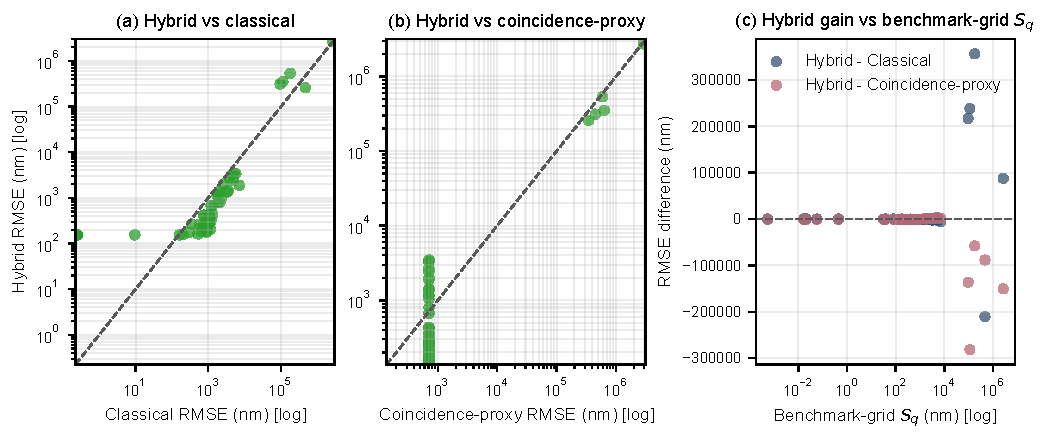
\includegraphics[width=0.98\textwidth]{paper_alicona_benchmark/figures/paired_method_comparison.pdf}
\caption{Per-surface paired comparison of measured-surface height RMSE. Panels (a) and (b) compare hybrid RMSE directly against the classical and quantum-like branches on the same surfaces; points below the dashed identity line favour the hybrid branch. Panel (c) shows the corresponding hybrid RMSE gain as a function of the FV reference $S_q$. Negative values favour hybrid reconstruction.}
\label{fig:alicona_pairwise}
\end{figure}
\unskip

A second architectural control separates coincidence-model effects from generic synthetic-wavelength behaviour. Table~\ref{tab:classical_two_color_control} compares the direct Q-diff branch and H-diff against a classical two-colour synthetic-wavelength baseline constructed from two classical PSI stacks at 810 and 809~nm. The direct long-$\Lambda$ behaviour is largely not quantum-specific: the classical two-colour baseline gives roughness medians comparable to or better than Q-diff on the matched-bandwidth grid, especially for $|\Delta S_z|$ (2346.7 versus 2879.5~nm), but it remains poor in pointwise height fidelity (1210.3 versus 710.0~nm). The key architectural result therefore survives at the hybrid level rather than at the direct long-$\Lambda$ branch itself: H-diff retains the lowest height RMSE (313.6~nm), whereas H-2-colour becomes competitive mainly for matched-bandwidth Sa and Sq bias. This control supports treating the coincidence-style channel as a useful coarse prior, but it weakens any claim that the direct envelope-descriptor benefit is uniquely quantum.

% Auto-generated by scripts/run_paper_classical_two_color_control.py
\begin{table}[t]
\centering
\footnotesize
\setlength{\tabcolsep}{4pt}
\caption{Auxiliary full-dataset control separating generic synthetic-wavelength behaviour from the coincidence-model branch over $n=59$ measured surfaces. The classical two-colour control uses two classical PSI stacks at 810 and 809~nm with the total classical photon budget split evenly between wavelengths. Reported values are medians of surface-level medians; roughness biases are referenced to the matched-bandwidth benchmark grid after area-averaged downsampling.}
\label{tab:classical_two_color_control}
\resizebox{\textwidth}{!}{%
\begin{tabular}{lccccc}
\toprule
Endpoint & Classical & Classical 2-colour & Q-diff & H-2-colour & H-diff \\
\midrule
Height RMSE (nm) & $1051.4$ & $1210.0$ & $710.0$ & $841.2$ & $313.4$ \\
$|\Delta S_a|$ (nm) & $333.3$ & $266.0$ & $332.7$ & $70.3$ & $87.0$ \\
$|\Delta S_q|$ (nm) & $439.5$ & $317.8$ & $398.2$ & $134.7$ & $153.0$ \\
$|\Delta S_z|$ (nm) & $8280.7$ & $2562.5$ & $2826.6$ & $5275.8$ & $5219.5$ \\
\bottomrule
\end{tabular}
}%
\end{table}


That strengthened comparator can be pushed further. Table~\ref{tab:classical_frontier_control} forms an optimistic classical-frontier oracle by allowing each surface and endpoint to choose the best available classical workflow among the default PSI, least-squares unwrap, LSQ plus frame-normalisation, and classical two-colour controls. Even under that oracle, the classical family still does not close the main height-fidelity gap: the best classical frontier remains at 559.1~nm versus 314.0~nm for hybrid. The roughness picture is less flattering to the hybrid claim: the oracle classical frontier reaches lower median absolute biases for Sa, Sq, and Sz (74.2, 86.4, and 1208.2~nm) by switching workflows across surfaces. The defensible claim is therefore narrower than universal hybrid dominance over every endpoint. What survives the strengthened comparator is that hybrid remains the strongest fixed-workflow height-fidelity architecture, while roughness leadership across the broader classical family remains endpoint- and workflow-dependent.

% Auto-generated by scripts/run_paper_classical_frontier_control.py
\begin{table}[t]
\centering
\footnotesize
\setlength{\tabcolsep}{4pt}
\caption{Classical-frontier control over $n=59$ measured surfaces. The table compares the default classical paper workflow, a classical least-squares unwrap, a stronger classical least-squares plus frame-normalised workflow, and a classical two-colour synthetic-wavelength baseline. The `Best classical frontier (oracle)` column is an optimistic upper bound formed by taking the per-surface minimum for each endpoint across these classical baselines and then reporting the resulting dataset median; it is therefore not a single deployable workflow. The final column shows the main hybrid branch for reference.}
\label{tab:classical_frontier_control}
\resizebox{\textwidth}{!}{%
\begin{tabular}{lcccccc}
\toprule
Endpoint & Classical default & Classical LS unwrap & Classical LSQ + norm & Classical 2-colour & Best classical frontier (oracle) & Hybrid \\
\midrule
Height RMSE (nm) & $1065.7$ & $559.2$ & $559.1$ & $1209.9$ & $559.1$ & $314.0$ \\
$|\Delta S_a|$ (nm) & $301.8$ & $366.3$ & $366.8$ & $265.4$ & $74.2$ & $129.6$ \\
$|\Delta S_q|$ (nm) & $423.4$ & $729.4$ & $728.4$ & $316.8$ & $84.7$ & $419.1$ \\
$|\Delta S_z|$ (nm) & $37163.2$ & $43202.2$ & $43198.0$ & $2278.5$ & $1368.5$ & $37457.4$ \\
\bottomrule
\end{tabular}
}%
\end{table}


The same split is visible in the spatial-frequency domain. Figure~\ref{fig:psd_representative} shows the radial power spectral density (PSD) on two representative measured surfaces reconstructed by the three pipelines on the common benchmark grid: a smoother ground stainless-steel surface and a rougher turned Ti-6Al-4V surface. Across both panels, classical PSI and the hybrid branch remain closer to the reference spectrum into the higher spatial-frequency region, whereas the direct quantum-like reconstruction follows the lower-frequency envelope more strongly than the fine-texture tail. This frequency-domain view is consistent with the metric-level result that the coincidence-like channel can remain useful for broader envelope descriptors while still losing fine-scale fidelity.

\begin{figure}[t]
\centering
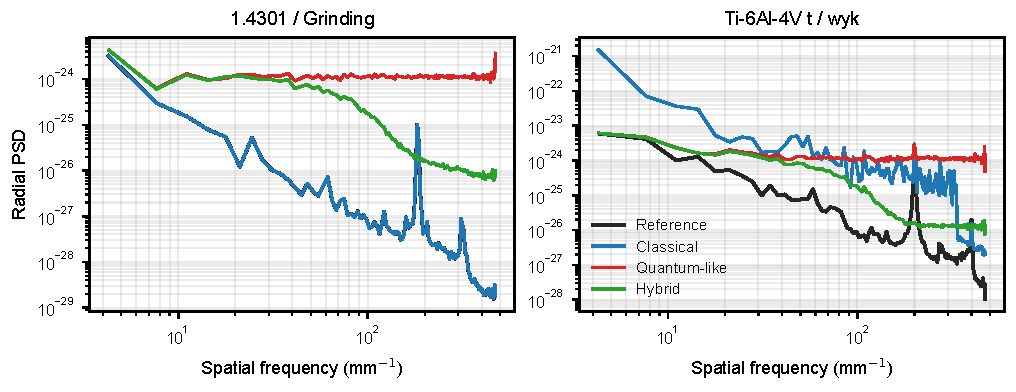
\includegraphics[width=0.98\textwidth]{paper_alicona_benchmark/figures/psd_representative.pdf}
\caption{Representative radial PSD comparison for two measured surfaces on the common benchmark grid: a smoother ground stainless-steel surface (left) and a rougher turned Ti-6Al-4V surface (right). The reference is the downsampled interferometric input surface after detrending. In both cases classical PSI and the hybrid reconstruction remain closer to the reference over the higher spatial-frequency tail, whereas the direct quantum-like reconstruction follows the lower-frequency envelope more strongly than the fine-texture content.}
\label{fig:psd_representative}
\end{figure}
\unskip

Figure~\ref{fig:alicona_residual_maps} complements those aggregate diagnostics with spatial residual maps for three automatically selected measured-surface cases: the surface with the lowest hybrid RMSE in the benchmark, the surface whose hybrid RMSE is closest to the dataset median, and the surface with the strongest direct quantum-like failure relative to the other branches. The same regime split remains visible in the image domain. In the low-error case, classical PSI and the hybrid branch keep the residual field locally structured and small, whereas the direct quantum-like reconstruction already shows broader envelope-scale distortion. In the mid-regime case, the hybrid branch visibly reduces the large-scale offset pattern relative to the direct quantum-like branch while remaining closer to the fine texture than the long-$\Lambda$ inversion. In the direct-Q-failure case, the residual field confirms that the difference-wavelength branch can fail catastrophically even when the classical and hybrid solutions remain well behaved.

\begin{figure}[t]
\centering
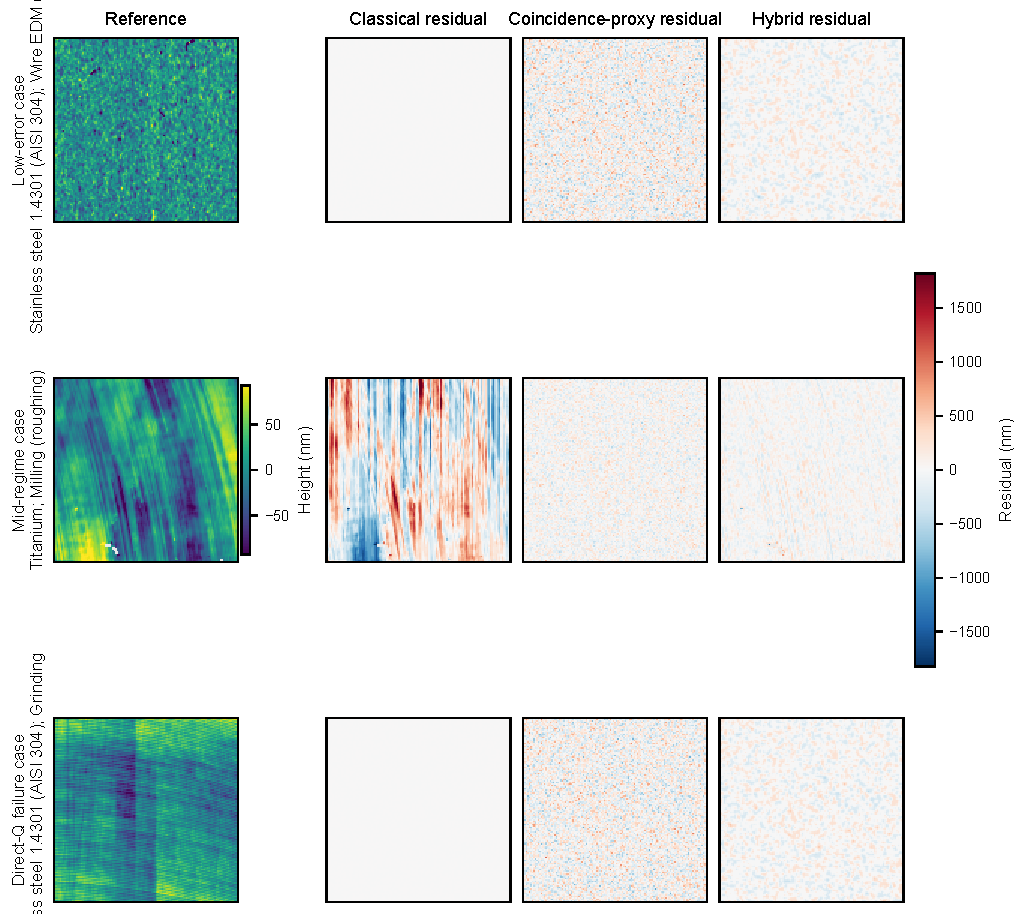
\includegraphics[width=0.90\textwidth]{paper_alicona_benchmark/figures/residual_maps_representative.pdf}
\caption{Representative measured-surface residual maps for three automatically selected benchmark cases. Rows correspond to the lowest-hybrid-error case, the surface whose hybrid RMSE is closest to the dataset median, and the surface with the largest direct quantum-like failure ratio relative to the classical/hybrid baselines. Columns show the downsampled benchmark surface used for the forward simulation and the residual maps for the classical, quantum-like, and hybrid reconstructions. The figure makes the image-domain consequence of the regime split explicit: the direct long-$\Lambda$ branch develops broader residual structures well before the hybrid branch loses the short-wavelength texture.}
\label{fig:alicona_residual_maps}
\end{figure}
\unskip

\begin{figure}[t]
\centering
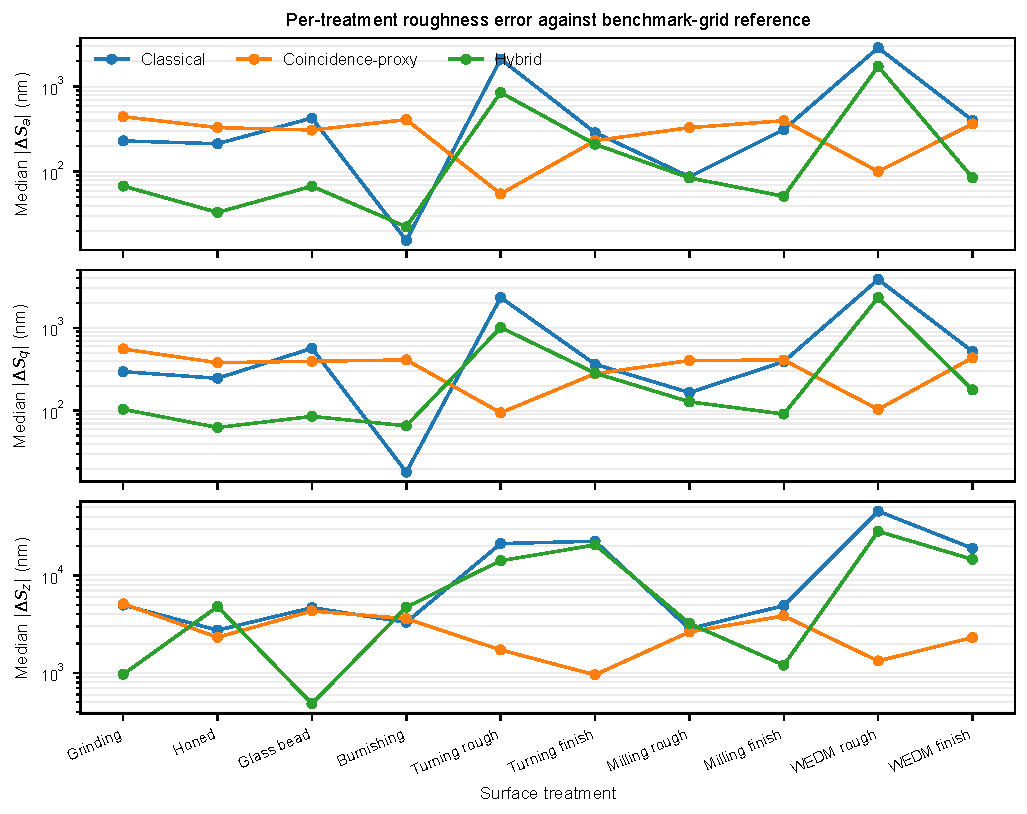
\includegraphics[width=0.98\textwidth]{paper_alicona_benchmark/figures/roughness_measured_by_treatment.pdf}
\caption{Median absolute roughness-parameter error split by surface treatment for the Alicona benchmark. Each panel reports the per-treatment median of $|\Delta S_a|$, $|\Delta S_q|$, or $|\Delta S_z|$ across measured \texttt{.sur} surfaces. The treatment view makes the process dependence explicit: hybrid reconstruction is typically strongest for Sa and Sq, while the quantum-like branch is only selectively favoured for Sz on smoother finishing treatments.}
\label{fig:alicona_roughness_by_treatment}
\end{figure}
\unskip

Because the forward model operates on a downsampled benchmark grid whereas the FV roughness reference remains native-grid, a full-dataset grid-sensitivity control was added at $128\times 128$, $256\times 256$, and $384\times 384$. Figure~\ref{fig:alicona_resolution_sensitivity} reports the corresponding dataset-level medians for height RMSE and absolute roughness bias. The absolute values shift with grid choice, as expected. Across the full dataset, hybrid remains the lowest-median branch for pointwise height RMSE at every tested grid (272.6, 314.0, and 303.5~nm), whereas the quantum-like branch remains nearly flat around 710~nm and the classical branch varies strongly with resolution. For roughness bias the ordering is metric dependent: hybrid improves further for $|\Delta S_a|$ and $|\Delta S_q|$ at $384\times 384$, while the direct quantum-like $|\Delta S_z|$ advantage persists across the tested grids. This control does not remove the native-grid versus benchmark-grid mismatch, but it does show that the central hybrid height-fidelity advantage is not created solely by the default $256\times 256$ simulation grid.

\begin{figure}[t]
\centering
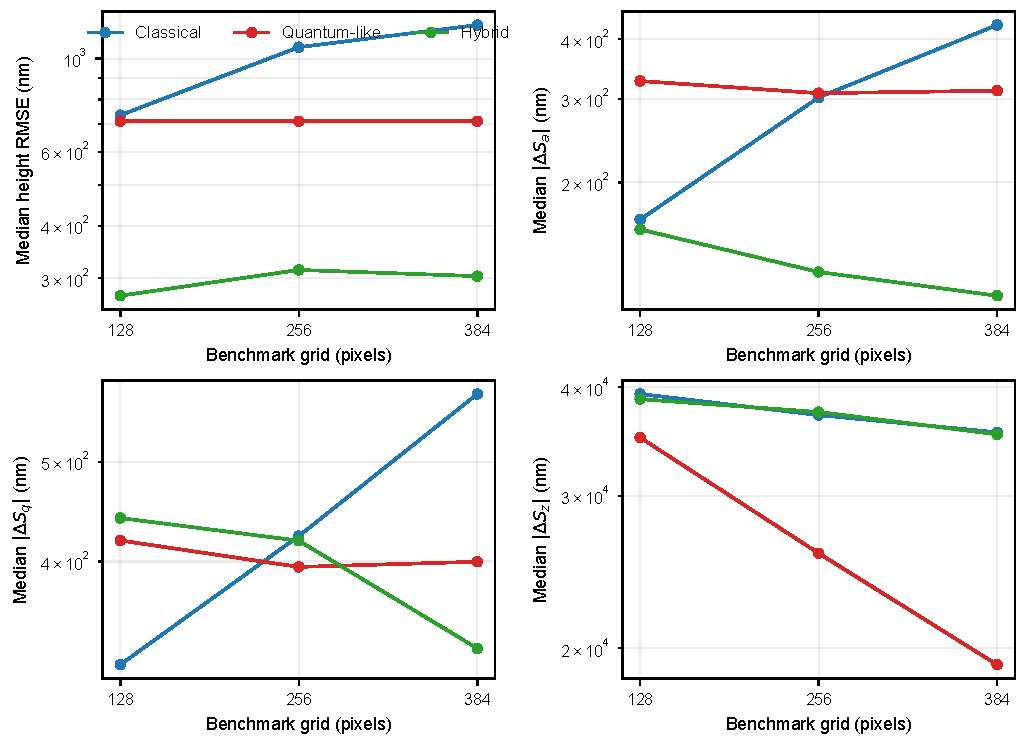
\includegraphics[width=0.94\textwidth]{paper_alicona_benchmark/figures/resolution_sensitivity_summary.pdf}
\caption{Sensitivity of the measured-surface benchmark to the downsampled simulation-grid resolution over the full dataset. The benchmark is rerun at $128\times 128$, $256\times 256$, and $384\times 384$, and the panels report the corresponding dataset-level medians for height RMSE and absolute roughness bias. The control is intended to expose dependence on the benchmark grid, not to redefine the native-grid FV reference.}
\label{fig:alicona_resolution_sensitivity}
\end{figure}
\unskip

Table~\ref{tab:benchmark_unwrap_control} adds a second dataset-level control for the direct branches: the full measured-surface benchmark is rerun with a global least-squares Poisson unwrap instead of the default separable row/column unwrap. The hybrid branch is unchanged by construction because its fringe-order assignment is driven directly by the coarse coincidence prior rather than by a full-map unwrap of the short-wavelength phase. The control does not leave all direct-branch medians unchanged: the global least-squares unwrap lowers classical height RMSE from 1065.7 to 559.2~nm, but it also worsens the classical roughness-bias endpoints to 366.3, 729.4, and 43202.2~nm for $|\Delta S_a|$, $|\Delta S_q|$, and $|\Delta S_z|$, respectively, and leaves the direct quantum-like branch essentially unchanged. Hybrid therefore remains the lowest-median height-fidelity branch overall, and the control does not overturn the architectural reading that the coincidence channel is more defensible as a coarse prior than as a direct final estimator.

% Auto-generated by scripts/run_paper_unwrap_control.py
\begin{table}[t]
\centering
\footnotesize
\setlength{\tabcolsep}{4pt}
\caption{Measured-surface unwrapping control over the full benchmark dataset. Direct classical and quantum-like branches are rerun with a global least-squares Poisson unwrap instead of the default separable row/column unwrap; entries report surface-level medians after collapsing repeated runs within each surface and method. The hybrid branch is unchanged because it uses the coincidence-derived coarse prior directly for fringe-order assignment.}
\label{tab:benchmark_unwrap_control}
\resizebox{\textwidth}{!}{%
\begin{tabular}{lccccc}
\toprule
Endpoint & Classical (simple) & Classical (least-squares) & Quantum-like (simple) & Quantum-like (least-squares) & Hybrid \\
\midrule
Height RMSE (nm) & $1065.7$ & $559.2$ & $709.6$ & $710.2$ & $314.0$ \\
$|\Delta S_a|$ (nm) & $301.8$ & $366.3$ & $308.1$ & $311.5$ & $129.6$ \\
$|\Delta S_q|$ (nm) & $423.4$ & $729.4$ & $395.2$ & $397.6$ & $419.1$ \\
$|\Delta S_z|$ (nm) & $37163.2$ & $43202.2$ & $25745.5$ & $25041.7$ & $37457.4$ \\
\bottomrule
\end{tabular}
}%
\end{table}


Table~\ref{tab:benchmark_rate_model_control} then promotes the stronger coincidence forward model into the full measured-surface branch. The ideal matched-count rate model is useful as an internal check: it lowers the direct quantum-like median height RMSE from 709.6 to 355.1~nm and the hybrid median from 314.0 to 290.9~nm, so the simple proxy is not artificially optimistic for the coincidence channel on the main height-fidelity endpoint. For practical interpretation, however, the non-ideal rate setting is the more conservative benchmark. Once accidentals, efficiency imbalance, and deadtime are added in the same rate framework, the direct coincidence-proxy branch becomes the most fragile path again, with median height RMSE rising to 1308.3~nm and $|\Delta S_a|$ to 741.9~nm, whereas the hybrid branch degrades more modestly to 376.3~nm and 184.7~nm. The rate-model control therefore exposes a real deployment risk for direct coincidence-only reconstruction while preserving the narrower architectural reading: coincidence information can still be useful, yet it is more defensible as a coarse prior than as the sole final estimator on rough measured surfaces.

% Auto-generated by scripts/run_paper_measured_rate_control.py
\begin{table}[t]
\centering
\footnotesize
\setlength{\tabcolsep}{4pt}
\caption{Measured-surface rate-model control over the full benchmark dataset. The canonical simple coincidence proxy is compared against a matched-count rate model and a non-ideal rate model with accidentals, detector-efficiency imbalance, and nonparalyzable deadtime. The rate-model controls use a gate time of 1.000~ms; the non-ideal setting additionally uses $\tau_c=20.0$~ns, $\eta_1=0.70$, $\eta_2=0.50$, and deadtime $\tau_d=5.0$~ns in each arm. Entries report surface-level medians after collapsing repeated runs within each surface and method.}
\label{tab:benchmark_rate_model_control}
\resizebox{\textwidth}{!}{%
\begin{tabular}{lccccccc}
\toprule
Endpoint & Classical & Q-like (simple) & Q-like (rates) & Q-like (non-ideal rates) & Hybrid (simple) & Hybrid (rates) & Hybrid (non-ideal rates) \\
\midrule
Height RMSE (nm) & $1065.7$ & $709.6$ & $355.1$ & $1308.3$ & $314.0$ & $290.9$ & $376.3$ \\
$|\Delta S_a|$ (nm) & $301.8$ & $308.1$ & $142.3$ & $741.9$ & $129.6$ & $138.6$ & $184.7$ \\
$|\Delta S_q|$ (nm) & $423.4$ & $395.2$ & $262.2$ & $805.2$ & $419.1$ & $435.8$ & $362.3$ \\
$|\Delta S_z|$ (nm) & $37163.2$ & $25745.5$ & $26473.1$ & $23823.9$ & $37457.4$ & $37642.6$ & $37190.8$ \\
\bottomrule
\end{tabular}
}%
\end{table}


\subsection{Step-free optical-property sweep}
To isolate texture-fidelity effects from step-unwrapping effects, a second benchmark was carried out on step-free synthetic rough surfaces while varying the surface RMS, sample reflectivity $R$, and visibility scaling factor $V_\mathrm{scale}$. Table~\ref{tab:optprops_rmse_step0} summarises the corresponding height RMSE values. Two representative regimes are promoted into the main figure set in Figure~\ref{fig:optprops_rmse_rms}: a low-return case ($R=0.20$, $V_\mathrm{scale}=0.70$) and a high-return case ($R=1.00$, $V_\mathrm{scale}=1.00$).

Across both cases, the difference-wavelength coincidence proxy (Q-diff) and the associated hybrid (H-diff) are clearly suboptimal for texture reconstruction: as the effective wavelength becomes very long, nm-scale roughness produces only weak phase modulation, and the resulting height RMSE becomes orders of magnitude larger than for the classical baseline. By contrast, the NOON-like channel stays close to the classical solution at low roughness and becomes lower-RMSE in the rougher part of the high-return case. In the low-return scenario, classical PSI and H-noon2 remain the most stable fine-texture baselines. In the high-return case, Q-noon2 gives the lowest RMSE at $S_q=80$~nm, while H-noon2 becomes the best-performing branch at $S_q=120$~nm. Classical PSI is therefore not the universal winner across the synthetic sweep; the more defensible statement is that classical PSI and H-noon2 define the default fine-texture baseline at low-to-moderate roughness, whereas the NOON-like coincidence branches become competitive or superior only in the rougher step-free regime.

That reading is not a knife-edge consequence of choosing exactly 810/809~nm for the difference-wavelength proxy. Table~\ref{tab:optprops_lambda_sensitivity} perturbs the spacing around that design point and repeats the representative step-free $S_q\approx 80$~nm case at two visibility levels. Shortening the synthetic wavelength improves both Q-diff and H-diff, but even the best H-diff case remains far above classical PSI. The direct and hybrid difference-wavelength branches are therefore structurally poor for fine-texture recovery in this proxy model, not merely mistuned at the nominal 810/809 operating point.

The fairness question behind the matched-count comparison was also tested more broadly. Table~\ref{tab:optprops_budget_sensitivity} repeats the NOON-like step-free control in three representative regimes: a low-return / low-visibility case ($S_q\approx 49.4$~nm), the high-return transition case ($S_q\approx 79.0$~nm), and a rougher high-return case ($S_q\approx 118.5$~nm). Across all three, moving to matched detected counts consistently narrows the direct Q-noon2 gap to classical PSI without producing a hidden hybrid advantage. In the low-return case the direct-Q RMSE falls from 1.40 to 0.86~nm; in the transition high-return case it falls from 0.44 to 0.27~nm, and the same narrowing persists in the rougher high-return control. Classical PSI and H-noon2 remain numerically tied in all three zero-ambiguity scenarios. The result is therefore narrower than a claim of universal fair normalisation: budget convention matters quantitatively, and most strongly for the direct coincidence branch, but it does not change the architectural conclusion that hybrid advantage appears only when ambiguity handling is actually needed.

% Auto-generated by scripts/make_table_from_summary.py
\begin{table}[H]
\centering
\footnotesize
\setlength{\tabcolsep}{2.4pt}
\caption{Height RMSE (after plane detrending) for step-free surfaces. Entries are mean $\pm$ std over repeats; columns compare classical PSI with coincidence-proxy and hybrid pipelines for different interferometer models. Coherence model: Rayleigh (normal incidence).}
\label{tab:optprops_rmse_step0}
\resizebox{\textwidth}{!}{%
\begin{tabular}{rrrrr@{\,\ensuremath{\pm}\,}rr@{\,\ensuremath{\pm}\,}rr@{\,\ensuremath{\pm}\,}rr@{\,\ensuremath{\pm}\,}rr@{\,\ensuremath{\pm}\,}r}
\toprule
RMS (nm) & $R$ & $V_\mathrm{scale}$ & Model & \multicolumn{2}{c}{Classical} & \multicolumn{2}{c}{Q-diff} & \multicolumn{2}{c}{Q-noon2} & \multicolumn{2}{c}{H-diff} & \multicolumn{2}{c}{H-noon2} \\
\midrule
20 & 0.20 & 0.70 & rayleigh & $0.99$ & $0.01$ & $2497.12$ & $12.52$ & $1.54$ & $0.01$ & $488.38$ & $9.08$ & $0.99$ & $0.01$ \\
20 & 0.20 & 1.00 & rayleigh & $0.69$ & $0.00$ & $1740.47$ & $9.40$ & $1.08$ & $0.00$ & $344.16$ & $7.28$ & $0.69$ & $0.00$ \\
20 & 0.50 & 0.70 & rayleigh & $0.63$ & $0.00$ & $1575.25$ & $9.70$ & $0.97$ & $0.00$ & $313.90$ & $7.42$ & $0.63$ & $0.00$ \\
20 & 0.50 & 1.00 & rayleigh & $0.44$ & $0.00$ & $1100.05$ & $7.10$ & $0.68$ & $0.00$ & $224.27$ & $3.52$ & $0.44$ & $0.00$ \\
20 & 1.00 & 0.70 & rayleigh & $0.44$ & $0.00$ & $1113.35$ & $3.92$ & $0.69$ & $0.00$ & $226.48$ & $3.70$ & $0.44$ & $0.00$ \\
20 & 1.00 & 1.00 & rayleigh & $0.31$ & $0.00$ & $779.45$ & $3.35$ & $0.48$ & $0.00$ & $166.94$ & $2.01$ & $0.31$ & $0.00$ \\
50 & 0.20 & 0.70 & rayleigh & $3.21$ & $0.02$ & $4142.45$ & $18.64$ & $2.57$ & $0.02$ & $801.17$ & $11.32$ & $3.21$ & $0.02$ \\
50 & 0.20 & 1.00 & rayleigh & $2.24$ & $0.01$ & $2895.60$ & $19.12$ & $1.79$ & $0.01$ & $562.30$ & $9.31$ & $2.24$ & $0.01$ \\
50 & 0.50 & 0.70 & rayleigh & $2.03$ & $0.01$ & $2611.91$ & $13.41$ & $1.62$ & $0.01$ & $510.67$ & $10.98$ & $2.03$ & $0.01$ \\
50 & 0.50 & 1.00 & rayleigh & $1.42$ & $0.01$ & $1832.81$ & $7.13$ & $1.13$ & $0.01$ & $360.75$ & $4.90$ & $1.42$ & $0.01$ \\
50 & 1.00 & 0.70 & rayleigh & $1.43$ & $0.01$ & $1847.01$ & $13.81$ & $1.14$ & $0.00$ & $364.85$ & $6.73$ & $1.43$ & $0.01$ \\
50 & 1.00 & 1.00 & rayleigh & $1.01$ & $0.01$ & $1290.59$ & $6.66$ & $0.80$ & $0.00$ & $260.12$ & $3.56$ & $1.01$ & $0.01$ \\
80 & 0.20 & 0.70 & rayleigh & $269.57$ & $13.18$ & $10823.61$ & $69.28$ & $6.70$ & $0.03$ & $2076.79$ & $46.91$ & $36.00$ & $2.73$ \\
80 & 0.20 & 1.00 & rayleigh & $113.68$ & $18.01$ & $7492.62$ & $34.60$ & $4.65$ & $0.02$ & $1424.54$ & $32.32$ & $24.06$ & $1.39$ \\
80 & 0.50 & 0.70 & rayleigh & $90.55$ & $14.34$ & $6744.09$ & $24.02$ & $4.18$ & $0.02$ & $1304.21$ & $32.74$ & $21.23$ & $0.71$ \\
80 & 0.50 & 1.00 & rayleigh & $14.76$ & $2.82$ & $4694.14$ & $24.17$ & $2.92$ & $0.02$ & $903.91$ & $17.37$ & $13.29$ & $0.10$ \\
80 & 1.00 & 0.70 & rayleigh & $16.24$ & $4.45$ & $4759.62$ & $20.37$ & $2.94$ & $0.01$ & $926.70$ & $13.46$ & $13.45$ & $0.12$ \\
80 & 1.00 & 1.00 & rayleigh & $9.05$ & $0.04$ & $3311.49$ & $17.56$ & $2.05$ & $0.01$ & $644.98$ & $12.63$ & $9.05$ & $0.04$ \\
120 & 0.20 & 0.70 & rayleigh & $679.23$ & $34.95$ & $641548.26$ & $33806.91$ & $442.99$ & $25.03$ & $328753.02$ & $40420.69$ & $250.03$ & $39.50$ \\
120 & 0.20 & 1.00 & rayleigh & $647.71$ & $40.91$ & $458577.27$ & $24045.68$ & $383.11$ & $29.68$ & $212965.80$ & $21068.15$ & $224.90$ & $42.28$ \\
120 & 0.50 & 0.70 & rayleigh & $647.31$ & $25.57$ & $431383.12$ & $18481.55$ & $368.59$ & $15.63$ & $212453.07$ & $23982.84$ & $224.17$ & $20.38$ \\
120 & 0.50 & 1.00 & rayleigh & $683.85$ & $41.80$ & $241690.17$ & $15653.87$ & $250.04$ & $16.66$ & $101869.44$ & $18195.72$ & $154.64$ & $11.49$ \\
120 & 1.00 & 0.70 & rayleigh & $655.16$ & $41.76$ & $243936.99$ & $22033.98$ & $262.26$ & $20.09$ & $117074.30$ & $21171.13$ & $164.14$ & $30.20$ \\
120 & 1.00 & 1.00 & rayleigh & $636.67$ & $35.25$ & $85690.83$ & $8510.80$ & $137.23$ & $10.27$ & $34219.73$ & $3710.81$ & $109.61$ & $11.82$ \\
\bottomrule
\end{tabular}
}%
\end{table}

% Auto-generated by scripts/run_paper_lambda_visibility_sensitivity.py
\begin{table}[t]
\centering
\footnotesize
\setlength{\tabcolsep}{4pt}
\caption{Targeted wavelength-spacing and visibility sensitivity for a representative step-free rough surface ($S_q\approx 80$~nm) under the same cosine--Poisson proxy model used in the synthetic sweeps. Entries report mean $\pm$ std height RMSE over 10 noise realisations. The nominal paper operating point corresponds to $\Delta\lambda=1.0$~nm (810/809).}
\label{tab:optprops_lambda_sensitivity}
\resizebox{\textwidth}{!}{%
\begin{tabular}{ccccc}
\toprule
Visibility scale & $\Delta\lambda$ (nm) & $\Lambda_{\mathrm{eff}}$ ($\mu$m) & Classical RMSE (nm) & Quantum-like / Hybrid RMSE (nm) \\
\midrule
$0.70$ & $0.2$ & $3279.7$ & $18.5 \pm 6.0$ & $Q$: $23781.8 \pm 77.8$; $H$: $4522.2 \pm 41.6$ \\
 & $0.5$ & $1311.4$ & $18.5 \pm 6.0$ & $Q$: $9505.4 \pm 23.4$; $H$: $1804.5 \pm 8.4$ \\
 & $1.0$ & $655.3$ & $18.5 \pm 6.0$ & $Q$: $4751.7 \pm 16.2$; $H$: $906.9 \pm 10.3$ \\
 & $2.0$ & $327.2$ & $18.5 \pm 6.0$ & $Q$: $2379.3 \pm 6.6$; $H$: $457.7 \pm 4.5$ \\
\midrule
$1.00$ & $0.2$ & $3279.7$ & $9.1 \pm 0.0$ & $Q$: $16603.7 \pm 51.8$; $H$: $3159.0 \pm 27.1$ \\
 & $0.5$ & $1311.4$ & $9.1 \pm 0.0$ & $Q$: $6639.2 \pm 16.5$; $H$: $1264.4 \pm 11.0$ \\
 & $1.0$ & $655.3$ & $9.1 \pm 0.0$ & $Q$: $3324.7 \pm 11.3$; $H$: $638.4 \pm 8.8$ \\
 & $2.0$ & $327.2$ & $9.1 \pm 0.0$ & $Q$: $1664.1 \pm 5.5$; $H$: $326.0 \pm 3.7$ \\
\bottomrule
\end{tabular}
}%
\end{table}

% Auto-generated by scripts/run_paper_budget_sensitivity.py
\begin{table}[t]
\centering
\footnotesize
\setlength{\tabcolsep}{4pt}
\caption{Resource-normalisation sensitivity for three representative step-free NOON-like regimes. Entries report mean $\pm$ std height RMSE over 10 noise realisations. The scenarios span a low-return / low-visibility case, a high-return transition case, and a rougher high-return case; within each scenario the conventions compare the paper-default budget split, equal nominal source quanta per pixel, and matched detected counts in the coincidence proxy.}
\label{tab:optprops_budget_sensitivity}
\resizebox{\textwidth}{!}{%
\begin{tabular}{llccc}
\toprule
Scenario & Budget convention & Classical RMSE (nm) & Q-noon2 RMSE (nm) & H-noon2 RMSE (nm) \\
\midrule
Low return / low visibility ($S_q\approx 49.4$~nm, $R=0.20$, $V_\mathrm{scale}=0.70$) & Paper default & $0.79 \pm 0.00$ & $1.40 \pm 0.00$ & $0.79 \pm 0.00$ \\
 & Equal nominal quanta & $1.30 \pm 0.00$ & $1.40 \pm 0.00$ & $1.30 \pm 0.00$ \\
 & Equal detected counts & $0.79 \pm 0.00$ & $0.86 \pm 0.00$ & $0.79 \pm 0.00$ \\
\midrule
Transition high return ($S_q\approx 79.0$~nm, $R=1.00$, $V_\mathrm{scale}=1.00$) & Paper default & $0.25 \pm 0.00$ & $0.44 \pm 0.00$ & $0.25 \pm 0.00$ \\
 & Equal nominal quanta & $0.41 \pm 0.00$ & $0.44 \pm 0.00$ & $0.41 \pm 0.00$ \\
 & Equal detected counts & $0.25 \pm 0.00$ & $0.27 \pm 0.00$ & $0.25 \pm 0.00$ \\
\midrule
Rough high return ($S_q\approx 118.5$~nm, $R=1.00$, $V_\mathrm{scale}=1.00$) & Paper default & $0.25 \pm 0.00$ & $0.44 \pm 0.00$ & $0.25 \pm 0.00$ \\
 & Equal nominal quanta & $0.41 \pm 0.00$ & $0.44 \pm 0.00$ & $0.41 \pm 0.00$ \\
 & Equal detected counts & $0.25 \pm 0.00$ & $0.27 \pm 0.00$ & $0.25 \pm 0.00$ \\
\bottomrule
\end{tabular}
}%
\end{table}


\begin{figure}[t]
\centering
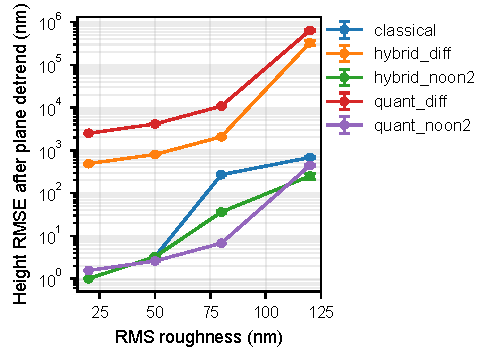
\includegraphics[width=0.48\textwidth]{paper_optprops_quick/figures/rmse_vs_rms__sc01.pdf}\hfill
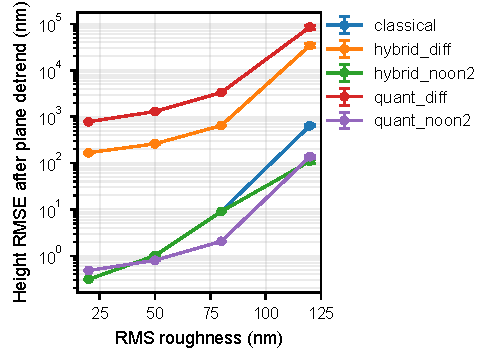
\includegraphics[width=0.48\textwidth]{paper_optprops_quick/figures/rmse_vs_rms__sc06.pdf}
\caption{Promoted optical-property sweep figures for the step-free case: height RMSE versus true surface roughness $S_q$ for two bounding sample conditions. Left: low reflectivity / low visibility ($R=0.20$, $V_\mathrm{scale}=0.70$). Right: high reflectivity / high visibility ($R=1.00$, $V_\mathrm{scale}=1.00$). These two panels are retained in the main paper because they bracket the optical-property range explored in Table~\ref{tab:optprops_rmse_step0} and make the method ordering visually explicit: classical PSI and H-noon2 define the low-to-moderate roughness baseline, the NOON-like branches become lower-RMSE in the rougher high-return regime, and Q-diff/H-diff sacrifice fine-texture fidelity in exchange for a large effective wavelength.}
\label{fig:optprops_rmse_rms}
\end{figure}
\unskip

\subsection{Targeted step / ambiguity regime control}
The step-free sweep above is intentionally blind to fringe-order ambiguity, so a complementary control was added on rough stepped surfaces with background roughness $S_q\approx 80$~nm and imposed vertical steps from 0 to 800~nm. Table~\ref{tab:optprops_step_sensitivity} and Figure~\ref{fig:optprops_step_sensitivity} report the absolute step-height error for low-return and high-return optical conditions. This control isolates the regime in which a long effective wavelength is valuable for metrology even though it is poor for fine-texture recovery.

In the high-return case, once the imposed step reaches 200~nm the long-$\Lambda$ branches clearly become the most accurate step estimators: the absolute step-height error drops from 270.8~nm for classical PSI to 40.7~nm for Q-diff and 38.4~nm for H-diff at 200~nm, and from 430.6~nm to 54.0~nm and 42.8~nm at 400~nm. The same pattern is noisier but still present in the low-return case, where at 600--800~nm Q-diff/H-diff stay within 116.4--224.1~nm and 155.1--161.6~nm, while classical PSI rises to 600.2--728.0~nm. By contrast, the NOON-like branches remain tied to the short-wavelength ambiguity burden and do not become the preferred step estimators once the discontinuity grows. The missing use-case from the step-free sweep is therefore explicit here: long-$\Lambda$ coincidence information is most useful when it is asked to resolve coarse discontinuity or fringe-order ambiguity, not when it is asked to carry the final fine-texture estimate.

% Auto-generated by scripts/run_paper_step_regime_control.py
\begin{table}[t]
\centering
\footnotesize
\setlength{\tabcolsep}{4pt}
\caption{Targeted ambiguity-regime control for a rough step surface with background roughness $S_q\approx 80$~nm. Entries report mean $\pm$ std absolute step-height error over 10 noise realisations while the imposed step height is varied. The two blocks bracket the low-return / low-visibility and high-return / high-visibility conditions used elsewhere in the paper.}
\label{tab:optprops_step_sensitivity}
\resizebox{\textwidth}{!}{%
\begin{tabular}{llccccc}
\toprule
Scenario & Step height (nm) & Classical & Q-diff & H-diff & Q-noon2 & H-noon2 \\
\midrule
Low return / low visibility ($R=0.20$, $V_\mathrm{scale}=0.70$) & 0 & $253.0 \pm 119.5$ & $184.3 \pm 80.4$ & $124.4 \pm 97.5$ & $7.9 \pm 5.0$ & $7.0 \pm 4.1$ \\
 & 100 & $129.1 \pm 121.1$ & $189.5 \pm 133.3$ & $170.7 \pm 114.7$ & $127.5 \pm 105.6$ & $150.6 \pm 129.4$ \\
 & 200 & $355.2 \pm 186.1$ & $162.6 \pm 140.5$ & $122.6 \pm 66.1$ & $207.6 \pm 8.2$ & $254.0 \pm 33.9$ \\
 & 300 & $269.4 \pm 149.7$ & $155.6 \pm 111.2$ & $142.3 \pm 83.6$ & $288.7 \pm 108.4$ & $306.9 \pm 92.4$ \\
 & 400 & $384.0 \pm 212.1$ & $250.2 \pm 147.0$ & $180.3 \pm 88.6$ & $410.1 \pm 8.0$ & $415.9 \pm 47.0$ \\
 & 600 & $600.2 \pm 238.0$ & $116.4 \pm 116.2$ & $155.1 \pm 78.5$ & $612.5 \pm 8.1$ & $546.6 \pm 8.4$ \\
 & 800 & $728.0 \pm 109.5$ & $224.1 \pm 122.5$ & $161.6 \pm 83.5$ & $814.7 \pm 8.0$ & $803.2 \pm 7.5$ \\
\midrule
High return / high visibility ($R=1.00$, $V_\mathrm{scale}=1.00$) & 0 & $7.8 \pm 4.9$ & $53.6 \pm 36.6$ & $45.5 \pm 31.7$ & $8.0 \pm 4.9$ & $7.8 \pm 4.9$ \\
 & 100 & $34.7 \pm 87.8$ & $50.2 \pm 28.0$ & $48.0 \pm 24.3$ & $88.9 \pm 108.1$ & $114.5 \pm 141.2$ \\
 & 200 & $270.8 \pm 8.1$ & $40.7 \pm 28.6$ & $38.4 \pm 30.9$ & $207.5 \pm 8.1$ & $263.2 \pm 28.0$ \\
 & 300 & $271.0 \pm 8.2$ & $70.1 \pm 45.4$ & $45.9 \pm 40.5$ & $288.5 \pm 110.6$ & $337.2 \pm 110.6$ \\
 & 400 & $430.6 \pm 136.5$ & $54.0 \pm 29.8$ & $42.8 \pm 26.1$ & $410.0 \pm 8.2$ & $443.5 \pm 63.7$ \\
 & 600 & $536.8 \pm 7.9$ & $44.7 \pm 35.9$ & $39.6 \pm 17.4$ & $612.4 \pm 8.2$ & $536.8 \pm 7.9$ \\
 & 800 & $803.0 \pm 7.9$ & $69.6 \pm 45.6$ & $52.4 \pm 20.2$ & $815.0 \pm 8.1$ & $803.0 \pm 7.9$ \\
\bottomrule
\end{tabular}
}%
\end{table}


\begin{figure}[t]
\centering
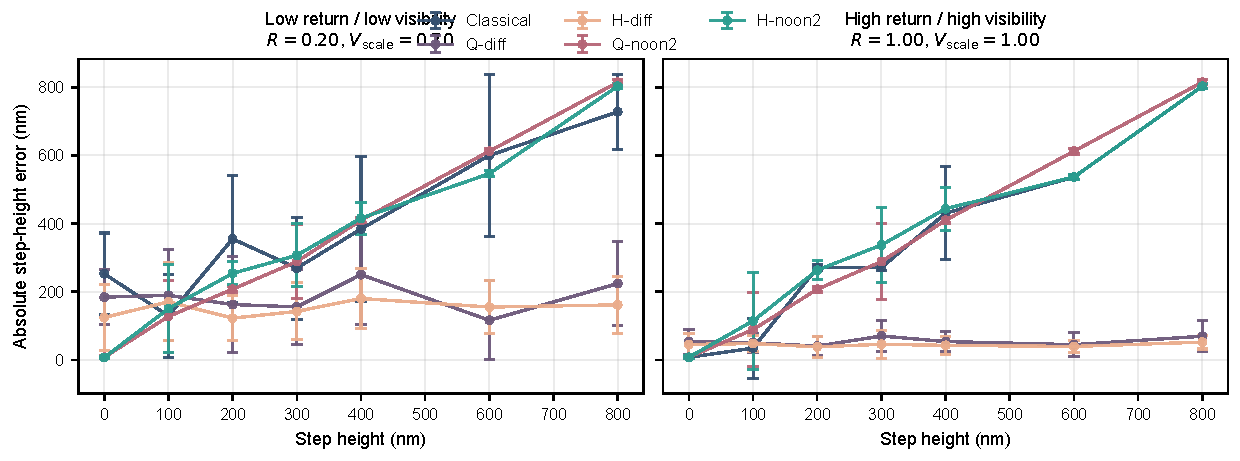
\includegraphics[width=0.82\textwidth]{paper_optprops_step_regime/step_regime_summary.pdf}
\caption{Targeted step/ambiguity control for rough stepped surfaces with background roughness $S_q\approx 80$~nm. The panels report absolute step-height error versus imposed step height for low-return and high-return conditions. The figure makes the architectural split explicit: long-$\Lambda$ difference branches become the best coarse step estimators once ambiguity enters, whereas the NOON-like and short-wavelength branches remain limited by fringe-order ambiguity.}
\label{fig:optprops_step_sensitivity}
\end{figure}
\unskip

\subsection{Targeted robustness check under phase-step jitter and frame drift}
Because coincidence-inspired channels are often discussed under idealised stepping conditions, a small targeted non-ideality stress test was added around the transition regime of Figure~\ref{fig:optprops_rmse_rms}. Rather than running a second full factorial campaign, one representative step-free case was selected at $R=1.00$, $V_\mathrm{scale}=1.00$, and $S_q=80$~nm, i.e., the point where the ordering between classical PSI and the NOON-like variants first becomes practically important. Three controls already supported by the simulator were then applied: Gaussian phase-step jitter with $\sigma_\delta=3^\circ$, frame-to-frame background and amplitude drift of $5\%$, and a mitigation control using least-squares reconstruction with frame-mean normalisation under the same drift.

% Auto-generated by scripts/make_nonideal_stress_artifacts.py
\begin{table}[t]
\centering
\footnotesize
\setlength{\tabcolsep}{5pt}
\caption{Representative non-ideality stress test for the step-free optical-property sweep at $R=1.00$, $V_\mathrm{scale}=1.00$, and true roughness $S_q=80$~nm. Entries are height RMSE mean $\pm$ std over 10 repeats. The first three rows use the baseline PSI4 reconstruction; the final row is a mitigation control using LSQ reconstruction with frame-mean normalisation under the same $5\%$ drift.}
\label{tab:optprops_nonideal_stress}
\begin{tabular}{lccc}
\toprule
Scenario & Classical & Q-noon2 & H-noon2 \\
\midrule
Baseline & $9.05 \pm 0.04$ & $2.05 \pm 0.01$ & $9.05 \pm 0.04$ \\
$+3^\circ$ phase-step jitter & $9.14 \pm 0.10$ & $2.12 \pm 0.08$ & $9.14 \pm 0.10$ \\
$+5\%$ background and amplitude drift & $133.40 \pm 93.39$ & $47.29 \pm 67.00$ & $71.78 \pm 36.07$ \\
Drift + LSQ + frame normalisation & $10.55 \pm 0.32$ & $2.28 \pm 0.16$ & $10.55 \pm 0.32$ \\
\bottomrule
\end{tabular}
\end{table}


\begin{figure}[t]
\centering
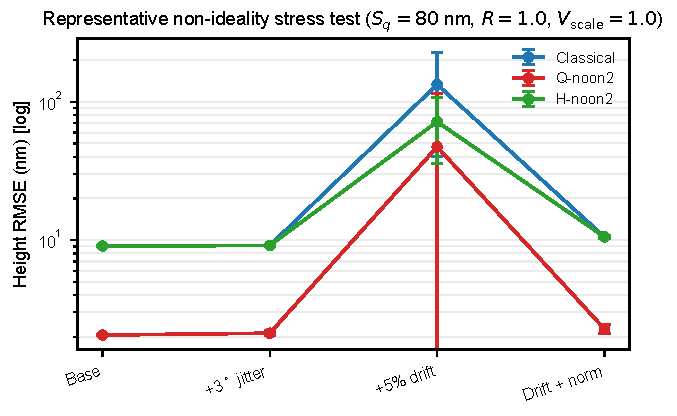
\includegraphics[width=0.66\textwidth]{paper_optprops_nonideal_stress/nonideal_stress_summary.pdf}
\caption{Representative non-ideality stress test for the step-free transition regime used in Table~\ref{tab:optprops_nonideal_stress}. The plot reports the same $R=1.00$, $V_\mathrm{scale}=1.00$, $S_q=80$~nm case for classical PSI, direct Q-noon2, and H-noon2. Moderate phase-step jitter perturbs the ranking only weakly, whereas frame drift produces the dominant degradation; the LSQ plus frame-normalisation control largely restores the baseline ordering in this representative case.}
\label{fig:optprops_nonideal_stress}
\end{figure}
\unskip

Table~\ref{tab:optprops_nonideal_stress} and Figure~\ref{fig:optprops_nonideal_stress} show that moderate phase-step jitter leaves the ranking essentially unchanged: the RMSE increase is about $1\%$ for classical PSI and H-noon2, and about $3\%$ for Q-noon2. By contrast, frame drift is the dominant non-ideality in this representative regime, inflating the RMSE to $133.4$~nm for classical PSI, $71.8$~nm for H-noon2, and $47.3$~nm for Q-noon2, with a marked rise in run-to-run variability. In the same moderate-roughness, high-return case, a simple LSQ plus frame-mean normalisation step largely restores near-baseline performance ($10.6$~nm, $2.28$~nm, and $10.6$~nm, respectively). This check is intentionally limited and should not be over-read as a full robustness map. Its value is narrower: within the present simulator, moderate phase-step jitter is not the principal failure mechanism, whereas frame drift is, and that drift is already tractable enough to justify including normalisation or active intensity stabilisation in any experimental follow-up.

\subsection{Detector-model sensitivity under matched mean coincidence counts}
Because the coincidence branch in the main benchmark is still represented by a simple phenomenological proxy, a second targeted check was added to the same step-free transition regime using the rate-based coincidence model under matched mean coincidence counts. The scenarios isolate a baseline rate model, a finite coincidence window, accidentals plus efficiency imbalance, and accidentals plus a nonparalyzable deadtime proxy; the gate time was fixed at $1$~ms and the quantum mean counts were matched to the simple proxy.

% Auto-generated by scripts/make_detector_sensitivity_artifacts.py
\begin{table}[t]
\centering
\footnotesize
\setlength{\tabcolsep}{5pt}
\caption{Representative detector-model sensitivity check for the step-free transition regime at $R=1.00$, $V_\mathrm{scale}=1.00$, and true roughness $S_q=80$~nm. The rate-based rows match the mean coincidence counts of the simple proxy using a 1.0~ms gate. Accidentals use a 20.0~ns coincidence window; the imbalance scenario additionally uses $\eta_1=0.70$ and $\eta_2=0.50$; the deadtime scenario uses a nonparalyzable 5.0~ns detector proxy. Entries are height RMSE mean $\pm$ std over 10 repeats.}
\label{tab:optprops_detector_sensitivity}
\begin{tabular}{lccc}
\toprule
Scenario & Classical & Q-noon2 & H-noon2 \\
\midrule
Simple coincidence proxy & $9.05 \pm 0.04$ & $2.05 \pm 0.01$ & $9.05 \pm 0.04$ \\
Rate model, matched mean counts & $9.05 \pm 0.04$ & $1.03 \pm 0.01$ & $9.05 \pm 0.04$ \\
Rate + accidentals & $9.05 \pm 0.04$ & $2.19 \pm 0.01$ & $9.05 \pm 0.04$ \\
Rate + accidentals + $\eta$ imbalance (0.70/0.50) & $9.05 \pm 0.04$ & $3.27 \pm 0.01$ & $9.05 \pm 0.04$ \\
Rate + accidentals + deadtime & $9.05 \pm 0.04$ & $2.46 \pm 0.01$ & $9.05 \pm 0.04$ \\
\bottomrule
\end{tabular}
\end{table}


\begin{figure}[t]
\centering
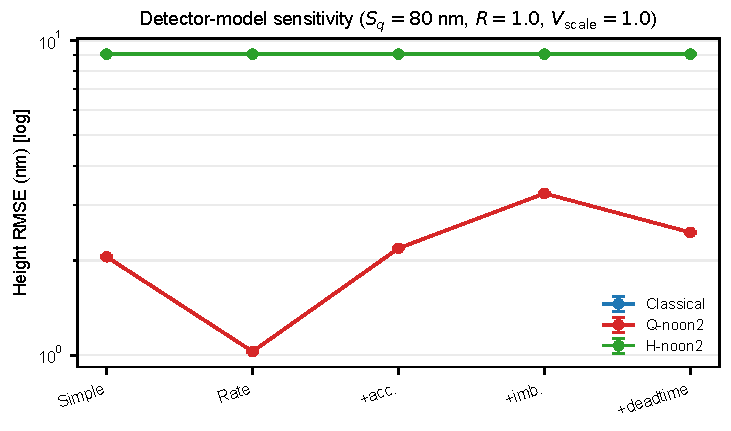
\includegraphics[width=0.68\textwidth]{paper_optprops_detector_sensitivity/detector_sensitivity_summary.pdf}
\caption{Representative detector-side sensitivity check for the same step-free transition regime used in Table~\ref{tab:optprops_detector_sensitivity}. The plot isolates the simple proxy, a matched-count rate model, accidentals, accidentals plus efficiency imbalance, and accidentals plus a nonparalyzable deadtime proxy. This zero-step case isolates only direct-branch sensitivity: the hybrid branch remains identical to the classical solution because no fringe-order ambiguity must be resolved, so the figure does not validate hybrid robustness under active ambiguity handling.}
\label{fig:optprops_detector_sensitivity}
\end{figure}
\unskip

Table~\ref{tab:optprops_detector_sensitivity} and Figure~\ref{fig:optprops_detector_sensitivity} show that detector-side assumptions mainly perturb the direct Q-noon2 branch in this representative case. Relative to the matched-count rate baseline ($1.03$~nm), Q-noon2 increases to $2.19$~nm with accidentals, $3.27$~nm with additional efficiency imbalance, and $2.46$~nm with deadtime. Classical PSI and H-noon2 remain numerically unchanged here because the selected step-free case contains no fringe-order ambiguity, so the hybrid estimator collapses to the classical short-wavelength branch. The detector-side study is therefore not a claim of universal robustness; its narrower value is only to show that moderate detector non-idealities can erode the direct coincidence benefit before they materially alter the zero-step direct branch.

\section{Discussion}
The measured-surface benchmark and the controlled optical-property sweep show that rough-surface profilometry does not admit a single universal winner. In the step-free sweep, classical PSI and H-noon2 define the low-to-moderate-roughness fine-texture baseline, while the NOON-like coincidence branches become lower-RMSE in the rougher high-return regime. In that same sweep the long synthetic-wavelength difference channel is not advantageous: the enlarged unambiguous range is bought at the cost of much weaker sensitivity to nm-scale texture, which is why Q-diff and H-diff degrade as the effective wavelength dominates the inversion.

That regime split becomes sharper once ambiguity is reintroduced directly. Table~\ref{tab:optprops_step_sensitivity} and Figure~\ref{fig:optprops_step_sensitivity} show that the long-$\Lambda$ difference branches become the best coarse step estimators once the imposed discontinuity enters the ambiguous regime, especially under high return, whereas the NOON-like branches do not. This is exactly the architectural role suggested by the measured-surface benchmark: a long effective wavelength is valuable as a coarse ambiguity-resolving cue, but not as the channel that should carry the final fine-texture estimate.

The targeted stress test in Table~\ref{tab:optprops_nonideal_stress} and Figure~\ref{fig:optprops_nonideal_stress} adds an operational nuance to that picture. In the representative transition regime, modest phase-step jitter barely changes the ordering, whereas frame drift is the more serious non-ideality; at the same time, a simple frame-normalisation control already recovers near-baseline accuracy in that case. For experimental follow-up, that shifts the immediate engineering priority away from only sub-degree refinement of the phase-step actuator and toward illumination/background stabilisation together with explicit drift compensation in the reconstruction \cite{McDonnell2020,Ri2020,Medina2014,Kim2026}.

The detector-side sensitivity check in Table~\ref{tab:optprops_detector_sensitivity} and Figure~\ref{fig:optprops_detector_sensitivity} sharpens that engineering picture further. In the same representative regime, accidentals, efficiency imbalance, and deadtime mainly perturb the direct Q-noon2 branch, while the zero-step H-noon2 result remains pinned to the classical branch because no fringe-order ambiguity must be resolved. Table~\ref{tab:benchmark_rate_model_control} then asks the same question at the full measured-surface level. Under an ideal matched-count rate model the direct quantum-like median height RMSE improves to 355.1~nm and the hybrid to 290.9~nm, so the simple proxy is not hiding a stronger direct branch; even there, hybrid remains the best height-fidelity option. Once accidentals, efficiency imbalance, and deadtime are propagated through the same full-dataset control, the direct branch degrades to 1308.3~nm while the hybrid rises only to 376.3~nm. The narrower implication is therefore still architectural rather than triumphalist: a more physical count-formation model can shift the quantitative boundaries of the regime map, but moderate detector non-idealities erode direct coincidence-only gains faster than they erase the hybrid advantage.

The FV benchmark narrows the stronger coincidence claim further. Under the native-grid FV reference, the direct quantum-like channel remains selectively useful for $S_q$ and especially $S_z$, but the matched-bandwidth control shows that only the $S_z$ advantage survives once the roughness comparison is referenced to the same area-averaged benchmark grid as the forward model. The auxiliary classical two-colour control goes one step further: much of the direct long-$\Lambda$ envelope-following behaviour can be reproduced by a purely classical synthetic-wavelength baseline. The added classical-frontier oracle raises the comparator bar further still. Even when the best available classical workflow is selected per surface and endpoint, the hybrid branch retains the best median height RMSE, while the classical family recovers lower roughness-bias medians by switching between default, unwrap-stabilised, and two-colour baselines. The added wavelength-spacing control reinforces the same point from the synthetic side: changing $\Delta\lambda$ shifts the severity of the Q-diff/H-diff penalty, but it does not recover a fine-texture regime in which the long-$\Lambda$ difference channel rivals the short-wavelength classical baseline. The budget-sensitivity control adds a fairness caveat of a different kind: changing the resource-normalisation convention can move the direct NOON-like branch closer to or farther from the classical error floor, but it does not reverse the architectural reading that coincidence information is most defensible as a coarse prior rather than as a standalone fine-texture estimator. What remains distinctive in the present proxy benchmark is therefore not a unique direct long-$\Lambda$ superiority, and not universal hybrid superiority over every roughness endpoint, but the fact that the coincidence-driven hybrid still yields the lowest fixed-workflow height RMSE while the roughness endpoints remain workflow- and process-dependent. Figures~\ref{fig:alicona_roughness_summary}, \ref{fig:alicona_roughness_by_treatment}, and \ref{fig:alicona_pairwise}, together with Tables~\ref{tab:alicona_roughness_median_abs}, \ref{tab:alicona_roughness_median_abs_bw}, \ref{tab:classical_two_color_control}, \ref{tab:classical_frontier_control}, \ref{tab:optprops_lambda_sensitivity}, and \ref{tab:optprops_budget_sensitivity}, all support that narrower reading.

Accordingly, the practical recommendation in this paper should be read asymmetrically. If one fixed workflow must be chosen and the main endpoint is detrended height RMSE, the hybrid branch is the best-supported option within the present proxy benchmark. If the endpoint is roughness bias, no universal workflow recommendation is supported here: matched-bandwidth $S_a$ and $S_q$ favour hybrid within the three primary branches, but stronger classical controls and treatment holdouts prevent that from being promoted to a portable rule, while native-grid $S_z$ mostly reflects envelope following and still breaches descriptor-scaled tolerance bands on most surfaces. In that sense the roughness endpoints serve here as diagnostic boundary conditions on the height-fidelity claim rather than as independent proof of overall superiority.

The added image-domain and implementation controls narrow that interpretation further. The residual maps in Figure~\ref{fig:alicona_residual_maps} show that the failure of the direct long-$\Lambda$ branch is not only a summary-statistic effect; it appears as a visible broad-structure distortion in the reconstructed height field. The full-dataset grid-sensitivity and unwrap controls in Figure~\ref{fig:alicona_resolution_sensitivity} and Table~\ref{tab:benchmark_unwrap_control} do not erase the modelling caveats, but they do indicate that the main hybrid height-fidelity advantage is not generated solely by the particular $256\times 256$ benchmark grid or by the default separable unwrap.

% Reviewer-facing synthesis table for the main failure mechanisms discussed in the paper.
\begin{table}[t]
\centering
\footnotesize
\setlength{\tabcolsep}{4pt}
\caption{Failure-mode taxonomy distilled from the measured-surface benchmark and the targeted control experiments. The table is intended as a design-oriented synthesis: it identifies the dominant observable signature, the branch most exposed to the failure mode, the part of the paper where that mode is evidenced, and the corresponding design implication.}
\label{tab:failure_taxonomy}
\resizebox{\textwidth}{!}{%
\begin{tabular}{>{\RaggedRight\arraybackslash}p{0.18\textwidth}>{\RaggedRight\arraybackslash}p{0.20\textwidth}>{\RaggedRight\arraybackslash}p{0.13\textwidth}>{\RaggedRight\arraybackslash}p{0.19\textwidth}>{\RaggedRight\arraybackslash}p{0.24\textwidth}}
\toprule
Failure mode & Primary signature & Most exposed branch & Evidence in this paper & Design implication \\
\midrule
Long-$\Lambda$ texture suppression & Broad residual structures and poor fine-texture recovery despite enlarged ambiguity range & Q-diff, then H-diff & Figure~\ref{fig:alicona_residual_maps}, Table~\ref{tab:classical_two_color_control}, Table~\ref{tab:optprops_lambda_sensitivity} & Treat long-$\Lambda$ information as a coarse prior or envelope cue, not as the primary nm-scale texture estimator. \\
Ambiguity / unwrap failure & Step-height error rises once the short-wavelength branch must bridge larger discontinuities; direct unwrap choice changes full-dataset medians & Classical direct branch and direct coincidence branches & Table~\ref{tab:benchmark_unwrap_control}, Table~\ref{tab:optprops_step_sensitivity} & Prefer coarse-to-fine hybrid unwrapping or at least verify direct-branch claims against a global unwrap control. \\
Budget-convention sensitivity & Direct Q-noon2 moves toward or away from the classical floor when the resource normalisation is changed, while the hybrid ordering stays stable & Direct Q-noon2 & Table~\ref{tab:optprops_budget_sensitivity} & Phrase low-light or fair-budget claims as convention-sensitive; do not infer a universal resource advantage from one normalisation. \\
Frame drift dominance & Background / amplitude drift causes much larger degradation than modest phase-step jitter, but is partly reversible by normalisation & All phase-stepped branches under drift, especially direct estimators & Table~\ref{tab:optprops_nonideal_stress}, Figure~\ref{fig:optprops_nonideal_stress} & Prioritise illumination stabilisation and frame-normalised LSQ reconstruction ahead of only tightening the phase-step actuator. \\
Detector-side coincidence erosion & Accidentals, efficiency imbalance, and deadtime erode direct coincidence gains before they create a new hybrid win & Direct coincidence branch & Table~\ref{tab:optprops_detector_sensitivity}, Table~\ref{tab:benchmark_rate_model_control} & Propagate detector losses through the design model and judge coincidence channels mainly by whether they still help a hybrid estimator. \\
Selective envelope-only descriptor gain & Native-grid $S_z$ can look favourable even when descriptor-scaled tolerance exceedance remains high & Direct quantum-like branch & Table~\ref{tab:benchmark_tolerance_rates}, Table~\ref{tab:dominance_summary} & Interpret $S_z$ wins as selective envelope following, not as broad roughness-fidelity improvement. \\
\bottomrule
\end{tabular}
}%
\end{table}

Table~\ref{tab:failure_taxonomy} compresses the benchmark into the failure modes that matter instrumentally. Long-$\Lambda$ branches fail by texture suppression, short-wavelength direct branches fail by ambiguity, budget convention mainly shifts the apparent strength of the direct coincidence branch, frame drift dominates moderate phase-step jitter, detector non-idealities erode direct coincidence gains earlier than hybrid gains, and native-grid $S_z$ wins remain primarily envelope-following events. Framed this way, the paper is not only a ranking study; it is a screening map of which failure mode is acceptable for a given metrology task.

This distinction is important because it changes the level at which the coincidence-derived contribution should be judged. Much of the surrounding quantum and quantum-inspired sensing literature is framed in terms of phase sensitivity, enlarged unambiguous range, or idealised resolution arguments \cite{Kapale2007,Didomenico2004169,Jha2011,Sharma2022,Xu2024}. Those are valuable starting points, but they do not by themselves answer the metrology question addressed here: whether a given architecture improves the reconstructed surface map or the downstream texture descriptor that an engineer would actually report. By translating the comparison into endpoint-specific accuracy, uncertainty, failure incidence, and PSD fidelity on realistic measured surfaces, and by setting that comparison against the corresponding classical robustness literature \cite{Ri2020,Medina2014,DeGroot1997283,McDonnell2020,Okamoto2021}, the present study moves the contribution from abstract sensing potential to instrument-selection evidence inside an explicitly limited proxy benchmark.

Taken together, the grouped material, treatment, roughness-parameter, paired-effect, and dominance comparisons are sufficient to propose a practical selection rule rather than only a retrospective interpretation. If the target is the lowest detrended height RMSE on measured rough surfaces and one fixed workflow must be selected in advance, the hybrid branch is the strongest overall choice. If the target is roughness bias, the present benchmark does not justify a universal selection rule: matched-bandwidth $S_a$ and $S_q$ favour hybrid within the three primary fixed workflows, but stronger classical controls and treatment holdouts prevent those endpoints from carrying a portable recommendation, while native-grid $S_z$ mostly tracks broad-envelope following and still violates descriptor-scaled tolerances on most surfaces. If the target is step-free fine-texture recovery in the controlled optical-property sweep, classical PSI remains the default baseline, with H-noon2 effectively tied once the coincidence channel is used only as a coarse prior. The robust grouped RMSE tables add an important constraint to that rule: hybrid is the median-best measured-surface branch in four of six material groups and eight of ten treatment classes, while the direct quantum-like branch is the grouped winner mainly for brass, graphite, turning (roughing), and wire-EDM (roughing). Classical PSI remains indispensable as the short-wavelength reference and as the donor branch inside the hybrid estimator, but it is not the robust median winner in any grouped measured-surface slice. A direct quantum-like reconstruction is therefore most defensible only when a selective native-grid envelope descriptor, especially $S_z$, is the endpoint of interest rather than the lowest height RMSE or the most stable broad-surface default. If a broader synthetic-wavelength envelope estimate is all that is needed, the classical two-colour control shows that a coincidence-style channel is not uniquely required. Table~\ref{tab:regime_summary} states that design rule in compact form, while Figure~\ref{fig:method_selection_flow} condenses it into a visual method-selection flow.

Operationally, that selection rule depends on four decision variables that are observable before committing to a reconstruction strategy: the primary endpoint of interest (height RMSE versus $S_a$, $S_q$, or $S_z$), the roughness regime or process class of the surface, whether ambiguity-tolerant coarse-height information is needed, and whether short-wavelength fine-texture fidelity must be preserved. Framing the problem in terms of those variables helps make the method-selection flow in Figure~\ref{fig:method_selection_flow} more than a narrative summary; it becomes an explicit decision structure that can be followed analytically.

That regime map also suggests a secondary methodological opportunity: uncertainty-aware method selection from observable surface descriptors, consistent with recent AI-enabled work on measurement-technique preselection, calibrated surface-parameter prediction, and broader coordinate-metrology decision support \cite{kucharski2025multitask-b68,Kucharski2024,Wieczorowski2023}.

% Narrative design-rule table distilled from the present benchmark
\begin{table}[t]
\centering
\footnotesize
\setlength{\tabcolsep}{4pt}
\renewcommand{\arraystretch}{1.08}
\caption{Regime-oriented method recommendation distilled from the measured-surface benchmark and the step-free optical-property sweep. The table is intentionally selective: it states where the present evidence supports each architecture and where it does not.}
\label{tab:regime_summary}
\begin{tabularx}{\textwidth}{>{\RaggedRight\arraybackslash}p{2.6cm}>{\RaggedRight\arraybackslash}p{4.0cm}>{\RaggedRight\arraybackslash}p{2.5cm}>{\RaggedRight\arraybackslash}X}
\toprule
Target endpoint & Supported regime in the present data & Preferred method & Rationale from the benchmark \\
\midrule
Lowest detrended height RMSE and finest texture fidelity & Step-free low-to-moderate roughness recovery; rougher measured classes; Al 7075, Brass, Graphite, Steel C45; turning (roughing), milling (finishing), wire-EDM & Classical PSI or H-noon2 & Classical PSI remains the pointwise baseline, and H-noon2 is effectively tied in the zero-step low-to-moderate regime because the final texture is still carried by the short-wavelength branch. \\

Rougher high-return step-free roughness recovery & Step-free sweep at higher roughness with favourable optical return ($S_q\approx 80$--$120$~nm; high $R$, high $V_\mathrm{scale}$) & Q-noon2 or H-noon2 & In the synthetic high-return case the NOON-like branches become lower-RMSE than the classical baseline while still avoiding the severe texture loss seen in the long-$\Lambda$ difference channel. \\

Ambiguity-tolerant measurement without losing short-wavelength detail & Cases where a coarse absolute-height prior is useful; nonclassical auxiliary channel acceptable; $S_a$ is the priority descriptor & Hybrid coarse-to-fine & The coincidence-derived channel stabilizes fringe-order selection, while the final map still inherits the fine texture from the short-wavelength classical branch. \\

Envelope-dominated roughness descriptors & Smoother finishing-style regimes; stainless steel 1.4301, Titanium; honed, burnished, glass-bead-blasted, and turning (finishing) surfaces; $S_q$ or $S_z$ more important than the absolute lowest RMSE & Direct quantum-like, selectively & The coincidence-like channel can retain broader excursions strongly enough to reduce $S_q$/$S_z$ bias in some smoother regimes, but it is not the preferred default for overall height accuracy. \\

Long synthetic-wavelength direct inversion as a primary estimator & Rough process classes or any regime demanding fine nm-scale texture fidelity & Not recommended as the default & The enlarged unambiguous range is bought at the cost of weaker texture sensitivity, which is why the strongest failures in the present study occur in the direct long-$\Lambda$ branch. \\
\bottomrule
\end{tabularx}
\end{table}

\begin{figure}[t]
\centering
\resizebox{0.96\textwidth}{!}{% Practical method-selection flow derived from the grouped benchmark trends
\begin{tikzpicture}[x=1cm,y=1cm, font=\footnotesize, >=Stealth]
  \tikzset{
    head/.style={draw, rounded corners=3pt, fill=gray!14, align=center, text width=4.7cm, minimum height=0.95cm, inner sep=5pt},
    qbox/.style={draw, rounded corners=3pt, fill=gray!8, align=center, text width=3.35cm, minimum height=1.55cm, inner sep=5pt},
    mbox/.style={draw, rounded corners=3pt, fill=gray!3, align=left, text width=3.45cm, minimum height=1.95cm, inner sep=6pt},
    note/.style={draw, rounded corners=3pt, fill=gray!8, align=center, text width=8.8cm, minimum height=0.95cm, inner sep=5pt},
    line/.style={-Stealth, line width=0.85pt}
  }

  \node[head] (start) at (0,0) {\textbf{Method selection guide}\\Choose the branch that matches the metrology endpoint.};

  \node[qbox] (rmseq) at (-4.4,-2.2) {\textbf{Height fidelity}\\Lowest RMSE or best fine\\texture reproduction};
  \node[qbox] (hybq) at (0,-2.2) {\textbf{Coarse prior needed}\\Ambiguity tolerance, but\\keep classical fine detail};
  \node[qbox] (qq) at (4.4,-2.2) {\textbf{Envelope descriptors}\\$S_q$ or $S_z$ matters more than\\the very lowest RMSE};

  \node[mbox] (classic) at (-4.4,-5.0) {\textbf{Classical PSI}\\Default baseline\\Best fit for rougher classes: grinding, rough turning, milling finishing, wire EDM.};
  \node[mbox] (hybrid) at (0,-5.0) {\textbf{Hybrid}\\Best nonclassical compromise\\Use when $S_a$ matters or when coincidence information should only stabilise unwrapping.};
  \node[mbox] (quantum) at (4.4,-5.0) {\textbf{Quantum-like}\\Use selectively\\Most defensible on smoother finishing-style regimes and mainly for $S_q$/$S_z$.};

  \node[note] (fallback) at (0,-7.55) {If the regime is unclear, keep \textbf{classical} as the baseline and prefer \textbf{hybrid} over direct coincidence inversion.};

  \draw[line] (start) -- (rmseq);
  \draw[line] (start) -- (hybq);
  \draw[line] (start) -- (qq);

  \draw[line] (rmseq) -- (classic);
  \draw[line] (hybq) -- (hybrid);
  \draw[line] (qq) -- (quantum);

  \draw[line] (classic.south) -- (fallback.north -| classic);
  \draw[line] (hybrid.south) -- (fallback.north);
  \draw[line] (quantum.south) -- (fallback.north -| quantum);
\end{tikzpicture}}
\caption{Practical method-selection flow distilled from the grouped benchmark results. The flow does not claim a universal winner; it summarises when the present data support classical PSI, hybrid coarse-to-fine reconstruction, or a direct quantum-like channel as the more appropriate choice.}
\label{fig:method_selection_flow}
\end{figure}
\unskip

From a photonics perspective, the most promising architecture emerging from these results is not a standalone long-$\Lambda$ coincidence measurement used as a direct roughness estimator, but a coarse-to-fine hybrid in which the coincidence-derived channel resolves ambiguity or provides a stabilising absolute-height prior while the final fine texture is still carried by short-wavelength PSI. The classical two-colour control makes that interpretation stricter: broad-envelope following alone does not justify a quantum claim, because much of that behaviour is already reproducible with a purely classical synthetic-wavelength baseline. The strongest surviving contribution is therefore architectural and benchmark-level rather than triumphalist. The paper identifies which role remains defensible for coincidence-derived information after realistic texture endpoints and stronger classical controls are imposed, and that narrower reading is also the one most compatible with the current implementation trajectory of integrated quantum photonics and correlated-photon instrumentation \cite{Mahmudlu2023518,Labbe2025,Yin20221316}.

Beyond surface metrology itself, the phase-screen formulation used here may also be useful as a structured robustness benchmark for interferometric architectures that target extremely small phase or path-length perturbations, where stability, ambiguity handling, and readout design matter alongside nominal phase sensitivity \cite{AdvancedLIGO2015,AmelinoCamelia1999,Chou2017}.

To turn the main revision blocker into an executable follow-up rather than a vague future-work item, the submission snapshot now fixes a reduced experimental-validation subset and corresponding protocol. Table~\ref{tab:experimental_validation_subset} summarises the six core and two extended surfaces chosen to test the best-case hybrid claim, a representative median case, the strongest direct-branch failure, the grouped rough-turning and rough-WEDM exceptions, the classical two-colour non-uniqueness case, the detector-fragility case, and the strongest native-grid $S_z$ envelope-following case. The accompanying protocol requires repeated acquisition of the classical, classical two-colour, direct coincidence, and hybrid branches on the same field of view, together with matched-bandwidth reporting and an independent reference cross-check where available.

% Auto-generated by scripts/select_experimental_validation_subset.py
\begin{table}[t]
\centering
\scriptsize
\setlength{\tabcolsep}{3pt}
\caption{Prepared reduced experimental-validation subset for the next revision-critical laboratory follow-up. The core rows are the minimum set needed to challenge the main architectural claim on real coincidence measurements; the extended rows add the second grouped exception family and the strongest native-grid envelope-following case. Raw stems retain the original measurement-file identifiers, while the English material and treatment descriptions are given below each stem.}
\label{tab:experimental_validation_subset}
\begin{tabularx}{\textwidth}{>{\RaggedRight\arraybackslash}p{0.08\textwidth}>{\RaggedRight\arraybackslash}p{0.20\textwidth}>{\RaggedRight\arraybackslash}p{0.30\textwidth}X}
\toprule
Tier & Case & Selected surface & Purpose in reduced validation \\
\midrule
Core & Best hybrid height & \path{P1-1.4301_wedm_zgru}\newline{\scriptsize Stainless steel 1.4301 (AISI 304); Wire EDM (roughing)} & Anchor best-case replication of the main fixed-workflow height-RMSE claim. \\
Core & Median hybrid height & \path{P1-Ti6A14V_frez_zgr}\newline{\scriptsize Titanium; Milling (roughing)} & Anchor a typical-case replication near the benchmark median. \\
Core & Catastrophic direct-Q failure & \path{1.4301_szlifowane}\newline{\scriptsize Stainless steel 1.4301 (AISI 304); Grinding} & Demonstrate the failure mode that most strongly limits direct coincidence-only reconstruction. \\
Core & Turning-roughing exception & \path{P1-C45_t_zgrubne}\newline{\scriptsize Steel C45; Turning (roughing)} & Test one treatment family where the direct branch is a grouped height-RMSE exception. \\
Core & Two-colour non-uniqueness & \path{P1-1.4301_frez_zgrub}\newline{\scriptsize Stainless steel 1.4301 (AISI 304); Milling (roughing)} & Test whether the envelope-following claim can be reproduced by a purely classical synthetic-wavelength baseline. \\
Core & Detector fragility & \path{Graphite_szkielkowane}\newline{\scriptsize Graphite; Glass bead blasted} & Test whether realistic detector non-idealities hurt the direct branch more than the hybrid branch. \\
Extended & Wire-EDM roughing exception & \path{P1-Ti6A14V_wedm_zgru_1prz}\newline{\scriptsize Titanium; Wire EDM (roughing)} & Add the second grouped height-RMSE exception family from the manuscript. \\
Extended & Native-grid $S\_z$ envelope & \path{C45_t_wyk}\newline{\scriptsize Steel C45; Turning (finishing)} & Add a native-grid Sz case where the direct branch has its clearest envelope-following advantage. \\
\bottomrule
\end{tabularx}
\end{table}


\paragraph{Limitations of the benchmark.}
The present work remains a simulation study built on real measured topographies rather than an experimental coincidence-metrology demonstration. The coincidence branch is not yet derived from or validated against a laboratory fourth-order interference transfer function, and the strongest rate-based control is therefore a sensitivity bound rather than a closure of the underlying quantum optics. The FV surfaces are operational references, not traceable absolute truth standards: no independent instrument cross-check or ISO-style $S/L$ filtering is applied in the present results, and the roughness outcomes therefore inherit FV bandwidth and outlier sensitivity. In addition, the main roughness comparison spans two bandwidth domains because the FV descriptors are computed on the native grid whereas the forward model operates on a downsampled benchmark grid. The matched-bandwidth control partially repairs that mismatch, but it also shows that native-grid $S_q$ rankings do not transfer cleanly.

The generalisation limits are likewise narrow. The material/treatment holdouts are adequate for height RMSE but weak for roughness (50\% treatment-holdout agreement for $|\Delta S_a|$ and 0\% for $|\Delta S_q|$), so the roughness descriptors should be interpreted as process-dependent diagnostics rather than portable method-selection rules. The matched-count comparison is also only one fairness convention; detector efficiency, accidentals, and deadtime materially move the direct-branch numbers, which is why the non-ideal rate control should be read as the more conservative deployment-facing bound. Finally, the benchmark spans six materials and ten treatments but not polished optics, additively manufactured surfaces, or other fundamentally different texture families. The present evidence therefore supports only a screening conclusion: coincidence-derived information remains worth testing as a coarse ambiguity-resolving prior, but experimental validation and traceable reference studies are still required before stronger metrology claims can be made. The reduced subset and protocol in Table~\ref{tab:experimental_validation_subset} are intended to close exactly that weakest link first rather than to postpone it indefinitely.

%%%%%%%%%%%%%%%%%%%%%%%%%%%%%%%%%%%%%%%%%%
\section{Conclusions}
This simulation benchmark supports a narrower conclusion than claims of quantum-enhanced profilometry. Using 59 real focus-variation (FV) height maps exported as Mountains/DigitalSurf \texttt{.sur} files as measured geometric references, together with simulated classical and coincidence-style observations generated from those surfaces, the study shows that the most defensible role for the coincidence-derived channel is not direct coincidence-only estimation but coarse-to-fine assistance to a classical PSI reconstruction. In the step-free optical-property sweep, classical PSI and H-noon2 form the low-to-moderate-roughness baseline for fine-texture recovery, whereas the NOON-like proxy branches become lower-RMSE only in the rougher high-return regime; long difference-wavelength reconstructions remain generally unsuited to primary fine-roughness estimation because they trade sensitivity for ambiguity range. The complementary step/ambiguity control makes the corresponding use-case explicit: long-$\Lambda$ difference branches become the best coarse step estimators once the imposed discontinuity enters the ambiguous regime, but they remain poor carriers of the final fine-texture estimate. In the measured-surface benchmark, the strengthened repeated-run, material/treatment-holdout, and classical-frontier controls do not overturn the same architectural reading for the main height endpoint: the hybrid branch remains the strongest fixed-workflow height-fidelity outcome, with a surface-level median RMSE of 314.0~nm and 32 of 59 per-surface wins.

Within that narrowed scope, the strongest result is fixed-workflow height fidelity. The hybrid branch remains the best measured-surface architecture at 314.0~nm median RMSE and 32 of 59 per-surface wins, and the stronger rate-based coincidence model preserves the same ordering: under ideal matched-count rates the hybrid branch remains best at 290.9~nm, while under non-ideal detector assumptions it rises only to 376.3~nm as the direct branch degrades to 1308.3~nm. Roughness endpoints do not support a universal workflow rule. Matched-bandwidth $S_a$ and $S_q$ favour hybrid within the primary branches, but treatment holdouts and stronger classical controls prevent portable claims, while native-grid $S_z$ remains mainly an envelope-following diagnostic and still exceeds descriptor-scaled tolerances on most surfaces. The classical-frontier oracle therefore weakens any blanket hybrid claim for roughness while leaving the main architectural result intact: within the present benchmark, coincidence-derived information is best justified as an auxiliary ambiguity-resolving prior inside a hybrid estimator when height fidelity is the primary endpoint.

For future work, the next step is now concrete rather than generic. The current submission snapshot already fixes a reduced experimental-validation subset and protocol (Table~\ref{tab:experimental_validation_subset}) that target the best-case hybrid claim, a representative median case, the strongest direct-branch failure, the grouped rough-treatment exceptions, the classical two-colour non-uniqueness case, and detector fragility against an independent reference chain where available. That first-pass reduced campaign should precede any broader claim expansion: replace the present proxy-plus-rate-control hierarchy with an experimentally grounded fourth-order transfer function, propagate detector-side effects under laboratory-representative losses, accidentals, and phase-stepping imperfections, and then test whether the hybrid advantage survives on that reduced measured-surface subset. A second equally important step is to archive the exact benchmark snapshot publicly. If the coarse-to-fine advantage survives both transitions, then hybrid coincidence-assisted profilometry becomes a credible candidate for experimental photonic metrology rather than only a coincidence-proxy simulation result.

%%%%%%%%%%%%%%%%%%%%%%%%%%%%%%%%%%%%%%%%%%
%%%%%%%%%%%%%%%%%%%%%%%%%%%%%%%%%%%%%%%%%%
\vspace{6pt}

%%%%%%%%%%%%%%%%%%%%%%%%%%%%%%%%%%%%%%%%%%
\vspace{6pt} 

%%%%%%%%%%%%%%%%%%%%%%%%%%%%%%%%%%%%%%%%%%
%% optional
%\supplementary{The following supporting information can be downloaded at:  \linksupplementary{s1}, Figure S1: title; Table S1: title; Video S1: title.}

% Only for journal Methods and Protocols:
% If you wish to submit a video article, please do so with any other supplementary material.
% \supplementary{The following supporting information can be downloaded at: \linksupplementary{s1}, Figure S1: title; Table S1: title; Video S1: title. A supporting video article is available at doi: link.}

% Only used for preprtints:
% \supplementary{The following supporting information can be downloaded at the website of this paper posted on \href{https://www.preprints.org/}{Preprints.org}.}

% Only for journal Hardware:
% If you wish to submit a video article, please do so with any other supplementary material.
% \supplementary{The following supporting information can be downloaded at: \linksupplementary{s1}, Figure S1: title; Table S1: title; Video S1: title.\vspace{6pt}\\
%\begin{tabularx}{\textwidth}{lll}
%\toprule
%\textbf{Name} & \textbf{Type} & \textbf{Description} \\
%\midrule
%S1 & Python script (.py) & Script of python source code used in XX \\
%S2 & Text (.txt) & Script of modelling code used to make Figure X \\
%S3 & Text (.txt) & Raw data from experiment X \\
%S4 & Video (.mp4) & Video demonstrating the hardware in use \\
%... & ... & ... \\
%\bottomrule
%\end{tabularx}
%}

%%%%%%%%%%%%%%%%%%%%%%%%%%%%%%%%%%%%%%%%%%
\authorcontributions{Conceptualization, D.K.; methodology, D.K.; software, D.K.; validation, D.K.; formal analysis, D.K.; investigation, D.K.; resources, D.K.; data curation, D.K.; writing---original draft preparation, D.K.; writing---review and editing, D.K.; visualization, D.K.; supervision, D.K. The author has read and agreed to the published version of the manuscript.}

\funding{This research received no external funding.}

\institutionalreview{Not applicable.}

\informedconsent{Not applicable.}

\dataavailability{The project files used for this study contain the manuscript sources, simulation code, input \texttt{.sur} surfaces, and the generated benchmark artefacts cited in the paper. Canonical regeneration is driven by \path{scripts/run_paper_measured_benchmark.py}, \path{scripts/run_paper_optprops.py}, and \path{scripts/select_experimental_validation_subset.py}; targeted controls, canonical sources, output folders, and revision-support files are enumerated in \path{docs/submission_snapshot_manifest.md}. The exact submission snapshot also contains the reduced experimental-validation subset under \path{outputs/paper_alicona_benchmark/experimental_validation/} together with the accompanying protocol in \path{docs/experimental_validation_protocol.md}. Because these materials have not yet been deposited in a public archival repository, no persistent repository identifier can yet be cited. Until archival deposition is completed, the exact submission snapshot is available from the corresponding author upon reasonable request.}

%\durcstatement{Current research is limited to the [please insert a specific academic field, e.g., XXX], which is beneficial [share benefits and/or primary use] and does not pose a threat to public health or national security. Authors acknowledge the dual-use potential of the research involving xxx and confirm that all necessary precautions have been taken to prevent potential misuse. As an ethical responsibility, authors strictly adhere to relevant national and international laws about DURC. Authors advocate for responsible deployment, ethical considerations, regulatory compliance, and transparent reporting to mitigate misuse risks and foster beneficial outcomes.}

% Only for journal Nursing Reports
%\publicinvolvement{Please describe how the public (patients, consumers, carers) were involved in the research. Consider reporting against the GRIPP2 (Guidance for Reporting Involvement of Patients and the Public) checklist. If the public were not involved in any aspect of the research add: ``No public involvement in any aspect of this research''.}
%
%% Only for journal Nursing Reports
%\guidelinesstandards{Please add a statement indicating which reporting guideline was used when drafting the report. For example, ``This manuscript was drafted against the XXX (the full name of reporting guidelines and citation) for XXX (type of research) research''. A complete list of reporting guidelines can be accessed via the equator network: \url{https://www.equator-network.org/}.}
%
%% Only for journal Nursing Reports
%\useofartificialintelligence{Please describe in detail any and all uses of artificial intelligence (AI) or AI-assisted tools used in the preparation of the manuscript. This may include, but is not limited to, language translation, language editing and grammar, or generating text. Alternatively, please state that “AI or AI-assisted tools were not used in drafting any aspect of this manuscript”.}

\acknowledgments{Not applicable.}

\conflictsofinterest{The author declares no conflicts of interest.}

%%%%%%%%%%%%%%%%%%%%%%%%%%%%%%%%%%%%%%%%%%
%% Optional

%% Only for journal Encyclopedia
%\entrylink{The Link to this entry published on the encyclopedia platform.}

\abbreviations{Abbreviations}{
The following abbreviations are used in this manuscript:
\\
\noindent
\begin{tabular}{@{}ll}
PSI & Phase-shifting interferometry
\end{tabular}
}

%%%%%%%%%%%%%%%%%%%%%%%%%%%%%%%%%%%%%%%%%%
%% Optional
%\isPreprints{}{% This command is only used for ``preprints''.
\begin{adjustwidth}{-\extralength}{0cm}
%} % If the paper is ``preprints'', please uncomment this parenthesis.

\reftitle{References}

% Please provide the correct journal abbreviation (e.g. according to the “List of Title Word Abbreviations” http://www.issn.org/services/online-services/access-to-the-ltwa/).
% Citations and References in Supplementary files are permitted provided that they also appear in the reference list here. 

% References: external bibliography
\bibliography{references}

% If authors have biography, please use the format below
%\section*{Short Biography of Authors}
%\bio
%{\raisebox{-0.35cm}{\includegraphics[width=3.5cm,height=5.3cm,clip,keepaspectratio]{Definitions/author1.pdf}}}
%{\textbf{Firstname Lastname} Biography of first author}
%
%\bio
%{\raisebox{-0.35cm}{\includegraphics[width=3.5cm,height=5.3cm,clip,keepaspectratio]{Definitions/author2.jpg}}}
%{\textbf{Firstname Lastname} Biography of second author}

% For the MDPI journals use author-date citation, please follow the formatting guidelines on http://www.mdpi.com/authors/references
% To cite two works by the same author: \citeauthor{ref-journal-1a} (\citeyear{ref-journal-1a}, \citeyear{ref-journal-1b}). This produces: Whittaker (1967, 1975)
% To cite two works by the same author with specific pages: \citeauthor{ref-journal-3a} (\citeyear{ref-journal-3a}, p. 328; \citeyear{ref-journal-3b}, p.475). This produces: Wong (1999, p. 328; 2000, p. 475)

%%%%%%%%%%%%%%%%%%%%%%%%%%%%%%%%%%%%%%%%%%
%% for journal Sci
%\reviewreports{\\
%Reviewer 1 comments and authors’ response\\
%Reviewer 2 comments and authors’ response\\
%Reviewer 3 comments and authors’ response
%}
%%%%%%%%%%%%%%%%%%%%%%%%%%%%%%%%%%%%%%%%%%
\PublishersNote{}
%\isPreprints{}{% This command is only used for ``preprints''.
\end{adjustwidth}
%} % If the paper is ``preprints'', please uncomment this parenthesis.
\end{document}

